\documentclass{book}
\usepackage{amsmath}
\usepackage{graphicx}
\usepackage{siunitx}
\usepackage{doi}
\usepackage[numbers]{natbib}
\usepackage{hyperref}
\usepackage{eso-pic}
\usepackage{xcolor}
\usepackage{tikz}
\usepackage{comment}
\newcommand\BackgroundPic{%
\put(0,0){%
\parbox[b][\paperheight]{\paperwidth}{%
\vfill
\centering

\includegraphics[width=\paperwidth,height=\paperheight]{background.jpg}%
\vfill
}}}

\hypersetup{
    colorlinks=true,
    linkcolor=blue,
    citecolor=blue,
    urlcolor=blue
}

% Ghent style blue
\definecolor{ugentblue}{RGB}{30,76,154}

\begin{document}

\begin{titlepage}
    \AddToShipoutPicture*{\BackgroundPic}

    \begin{tikzpicture}[remember picture, overlay]
        \node[
            fill=ugentblue,
            fill opacity=0.80,
            text opacity=1,
            rounded corners=8pt,
            inner sep=20pt,
            minimum width=0.78\paperwidth,
            minimum height=0.34\paperheight,
            text width=0.68\paperwidth,
            align=center
        ] at (current page.center) {
            {\color{white}\fontsize{24}{28}\selectfont\bfseries
            Predictive \mbox{Maintenance}  for Fusion Devices\par}
            \vspace{1cm}
            {\color{white}\Large Leonardo Caputo\par}
            \vspace{0.4cm}
            {\color{white}\large PhD Thesis\par}
            \vspace{0.4cm}
            {\color{white}\normalsize Ghent University\par}
            {\color{white}\normalsize 2026\par}
        };
    \end{tikzpicture}

    \null
    \ClearShipoutPicture
\end{titlepage}

\tableofcontents
\chapter{Introduction}
GENERAL INTRO

\section{Physical principles of nuclear fusion}
\label{sec:physics_fusion}
Nuclear fusion is a nuclear reaction in which two light atomic nuclei combine to form a heavier nucleus, with a net release of energy resulting from the increase in binding energy per nucleon. This energy corresponds to the mass difference between the initial and final states and is governed by the mass--energy equivalence relation \(E = mc^2\).

Fusion does not occur simply when two nuclei collide. Because of their positive electric charge, nuclei repel each other through the Coulomb force. Fusion therefore requires sufficiently high kinetic energies to overcome this repulsion, typically achieved at extremely high temperatures where particles move at high velocities. Under such conditions, matter no longer exists in the form of a neutral gas, but instead transitions into an ionized state known as plasma.

A plasma consists of a collection of free electrons and ions, and is often referred to as the fourth state of matter. Unlike neutral gases, plasmas exhibit collective behaviour due to long-range electromagnetic interactions between charged particles. As a consequence, plasmas are highly conductive and strongly influenced by externally applied electric and magnetic fields. These interactions make the physical description of plasmas significantly more complex than that of conventional fluids, requiring a combination of kinetic and fluid models to capture their behaviour.

Despite the extreme conditions required, nuclear fusion is fundamental to life on Earth. It is the process powering the Sun and other stars, where gravitational confinement enables the conditions necessary for sustained fusion reactions. The energy produced in these reactions is ultimately responsible for the radiation that drives the Earth's climate and supports all known life.

In the context of controlled fusion, understanding plasma behaviour is essential, as confinement, stability, and energy transport are governed by these interactions. The following subsections introduce the key physical concepts underlying fusion processes, including nuclear binding energy, the Coulomb barrier, fusion reactions, and fusion cross sections. These elements provide the foundation for understanding the conditions required for fusion and motivate the selection of the deuterium--tritium reaction as the most viable candidate for near-term energy production.

\subsection*{Nuclear binding energy}
To explain the origin of energy release in nuclear fusion, it is necessary to introduce the concept of nuclear binding energy (NBE). The nuclear binding energy is defined as the energy required to disassemble a nucleus into its constituent nucleons. Equivalently, it represents the energy that binds the nucleons together within the nucleus.

The existence of nuclear binding energy is a consequence of the mass defect: the mass of a bound nucleus is lower than the sum of the masses of its individual nucleons. This difference in mass corresponds to an energy difference according to the mass--energy equivalence relation
\begin{equation}
\Delta E = \Delta m c^2,
\end{equation}
where \(\Delta E\) is the energy difference, \(\Delta m\) the mass defect, and \(c\) the speed of light. This relation implies that any decrease in mass between the initial and final states of a nuclear reaction results in a release of energy.

Figure~\ref{fig:nbe-curve} shows the average nuclear binding energy per nucleon as a function of the mass number for naturally occurring nuclei. The variation of this quantity reflects the balance between the attractive strong nuclear force and the repulsive Coulomb interaction between protons.

This curve directly explains the mechanisms of both nuclear fusion and fission. For light nuclei, the binding energy per nucleon increases with mass number, meaning that the formation of heavier nuclei results in a more tightly bound and therefore more stable configuration. For instance, the binding energy per nucleon of \({}^{4}\mathrm{He}\) is significantly higher than that of hydrogen isotopes such as \({}^{1}\mathrm{H}\), \({}^{2}\mathrm{H}\), and \({}^{3}\mathrm{H}\). As a result, fusion reactions involving these light nuclei lead to the formation of more stable products and the release of energy.

The binding energy per nucleon reaches a maximum around \({}^{56}\mathrm{Fe}\), corresponding to the most stable nuclei. For heavier nuclei, the binding energy per nucleon decreases with increasing mass number. Consequently, energy can be released either by fusing light nuclei or by splitting heavy nuclei into lighter, more stable fragments. The latter process is known as nuclear fission~\cite{freidberg2007plasma}.

\begin{figure}[htbp]
  \centering
  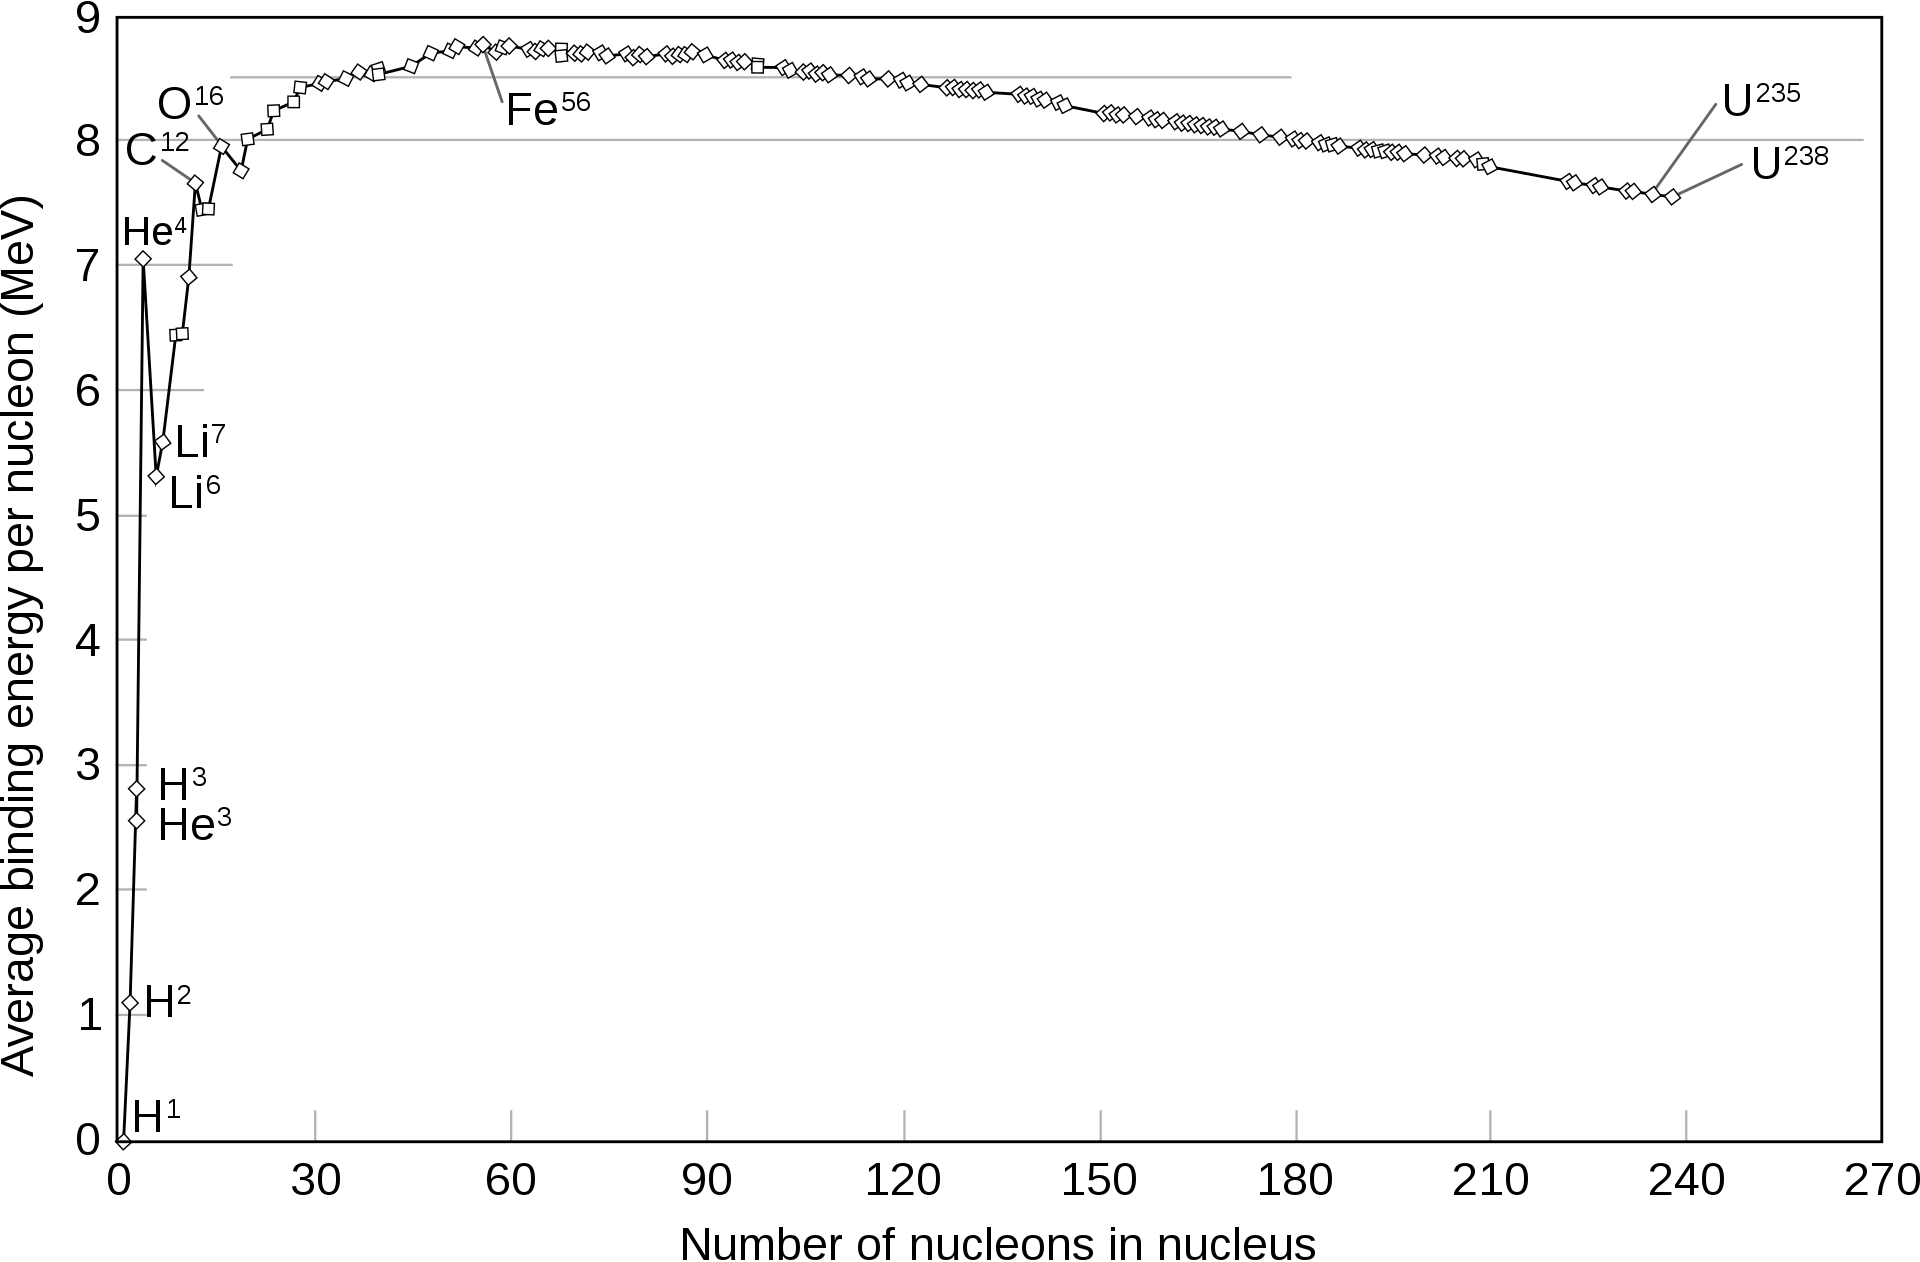
\includegraphics[width=0.85\linewidth]{Figures/nuclear_binding.png}
  \caption[Average nuclear binding energy per nucleon as a function of mass number]{Average nuclear binding energy per nucleon as a function of mass number. The curve illustrates the increase in stability for light nuclei up to iron (\(^{56}\mathrm{Fe}\)), beyond which fission becomes energetically favourable. Adapted from Lilley~\protect\cite{lilley2009nuclear}.}
  \label{fig:nbe-curve}
\end{figure}


\subsection*{Coulomb barrier}
Fusion does not occur simply when two nuclei collide. Because of their positive electric charge, nuclei repel each other through the Coulomb force. For fusion to take place, the interacting nuclei must approach each other closely enough for the attractive nuclear force to dominate. This requires that their relative kinetic energy is sufficient to overcome the Coulomb barrier.

The interaction between two nuclei can be described in terms of an effective potential resulting from the superposition of a short-range attractive nuclear potential and a long-range repulsive Coulomb potential. The resulting potential profile exhibits a maximum, referred to as the Coulomb barrier, which must be overcome or penetrated for fusion to occur. Figure~\ref{fig:coulomb} illustrates the qualitative shape of this interaction potential.

\begin{figure}[htbp]
  \centering
  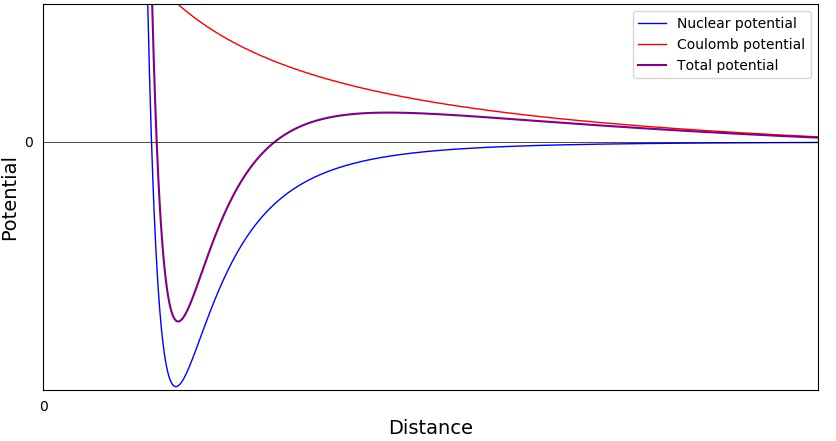
\includegraphics[width=0.85\linewidth]{Figures/coulomb_barrier.png}
  \caption{Schematic representation of the interaction potential between two nuclei, showing the repulsive Coulomb potential at large distances and the attractive nuclear potential at short distances. The resulting Coulomb barrier must be overcome or penetrated for fusion to occur. Adapted from~\cite{rousseau2019jet}.}
  \label{fig:coulomb}
\end{figure}

The height of the Coulomb barrier depends on the charges of the interacting nuclei and is proportional to the product \(Z_1 Z_2\), where \(Z_1\) and \(Z_2\) are the atomic numbers of the nuclei. As a result, nuclei with higher charge require significantly higher kinetic energies to reach the distances at which the nuclear force becomes dominant. For example, the Coulomb barrier for two helium nuclei is substantially higher than that for hydrogen isotopes. Consequently, fusion reactions involving light nuclei are more favourable, as they require lower energies to overcome the electrostatic repulsion.

\subsection*{Fusion reactions}
A variety of fusion reactions are possible, depending on the reacting nuclei. In all cases, the released energy appears primarily as kinetic energy of the reaction products. From the perspective of fusion energy, the most relevant reactions are those involving hydrogen isotopes, since they combine comparatively high reaction rates with relatively accessible ignition conditions.

Fusion in stars proceeds through chains of reactions in which hydrogen nuclei are progressively converted into helium. In the Sun, the dominant pathway is the proton proton chain. One of its final steps is
\begin{equation}
{}^{3}\mathrm{He} + {}^{3}\mathrm{He} \longrightarrow {}^{4}\mathrm{He} + 2p + \SI{12.86}{MeV}.
\tag{2.1}
\end{equation}
Although this reaction is of fundamental importance in stellar nucleosynthesis, it is not the most relevant for terrestrial fusion energy production. In particular, the Coulomb barrier for reactions involving \({}^{3}\mathrm{He}\) is substantially higher than for reactions involving hydrogen isotopes such as deuterium and tritium, and therefore much higher particle energies are required.

Among the simplest fusion reactions of practical interest are those involving deuterium (\(D\), \({}^{2}\mathrm{H}\)). The two dominant \(D\)–\(D\) branches are
\begin{equation}
D + D \longrightarrow {}^{3}\mathrm{He} + n + \SI{3.27}{MeV},
\tag{2.2}
\end{equation}
\begin{equation}
D + D \longrightarrow T + p + \SI{4.03}{MeV}.
\tag{2.3}
\end{equation}
A radiative branch is also possible,
\begin{equation}
D + D \longrightarrow {}^{4}\mathrm{He} + \gamma + \SI{23.85}{MeV},
\tag{2.4}
\end{equation}
but this reaction has a much lower probability than the two dominant channels above. The \(D\)–\(D\) reactions are of particular interest because deuterium is naturally abundant, but their reactivity remains lower than that of the deuterium tritium reaction at reactor relevant temperatures.

Of central importance for near term fusion energy research are the reactions involving fuel combinations with total mass number five:
\begin{equation}
D + T \longrightarrow {}^{4}\mathrm{He} + n + \SI{17.59}{MeV},
\tag{2.5}
\end{equation}
\begin{equation}
D + {}^{3}\mathrm{He} \longrightarrow {}^{4}\mathrm{He} + p + \SI{18.35}{MeV}.
\tag{2.6}
\end{equation}
Among these, the \(D\)–\(T\) reaction is the most important for present fusion reactor designs because it exhibits the highest reaction rate at the lowest temperature. For this reason, it is generally regarded as the most viable reaction for near term fusion energy production~\cite{freidberg2007plasma,stacey2018fusion}.

\subsection*{Fusion cross section}
Not every collision between nuclei with kinetic energy exceeding the Coulomb barrier results in a fusion reaction. Even when the barrier is overcome, fusion remains a probabilistic process due to the quantum mechanical nature of nuclear interactions. This probability is quantified by the fusion cross-section, which represents the effective area over which a fusion reaction can occur.

Figure~\ref{fig:xs} shows the fusion cross-sections for several reactions discussed in the previous subsection. The cross-section depends strongly on the relative kinetic energy of the interacting nuclei and varies significantly between different fusion reactions. In particular, cross-sections can differ by several orders of magnitude at comparable energies, which has important implications for the selection of suitable fusion fuels.

\begin{figure}[htbp]
  \centering
  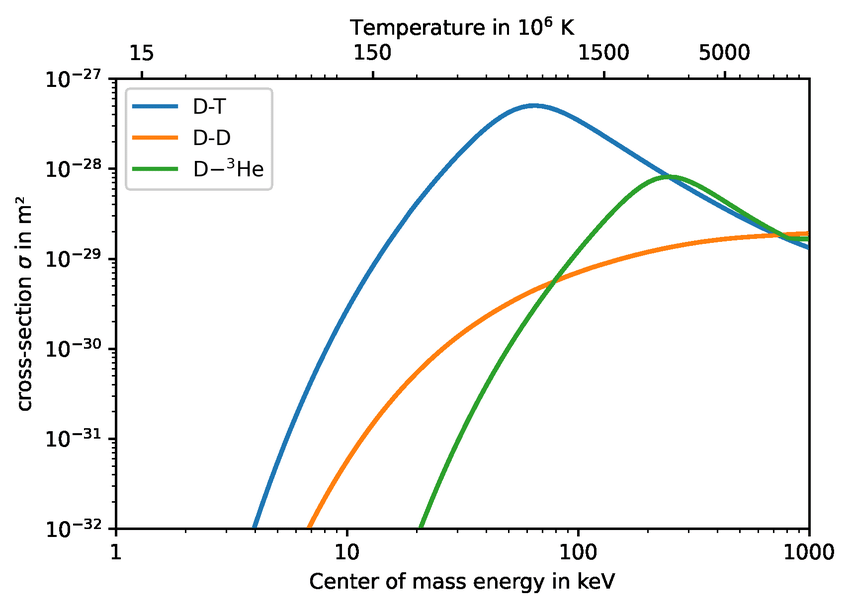
\includegraphics[width=0.85\linewidth]{Figures/cross_section_fusion.png}
  \caption{Fusion cross-sections as a function of particle energy for selected reactions. The strong dependence on energy and reaction type highlights the favourable characteristics of the \(D\)--\(T\) reaction compared to alternatives. Adapted from~\cite{freidberg2007plasma}.}
  \label{fig:xs}
\end{figure}

The strong variation in fusion cross-section directly influences reactor design, as it determines the temperature and confinement conditions required to achieve a sufficient reaction rate. In particular, the relatively high cross-section of the \(D\)--\(T\) reaction at attainable temperatures is a key reason for its selection in most current fusion reactor concepts.

\bigskip
\section{Engineering aspects of nuclear fusion}
\label{sec:Eng_fusion}


\subsection{Requirements for fusion}
This section discusses the main engineering requirements for achieving controlled nuclear fusion, including energy balance, plasma confinement, and reactor design considerations.

\paragraph{Breakeven and ignition.}
For fusion to be a viable energy source, the power generated by fusion reactions must at least compensate for the energy losses of the system. One of the dominant loss mechanisms in fusion plasmas is Bremsstrahlung radiation, which arises from the deceleration of electrons in the electric field of ions. These losses scale approximately with the square of the ion charge, highlighting the importance of maintaining a plasma composed of low-\(Z\) elements.

To sustain the plasma, external heating power is required to compensate for these losses. When the fusion power produced equals the externally supplied heating power, the system is said to reach breakeven. As the fusion power increases, a fraction of the released energy is transferred back to the plasma through charged fusion products, resulting in self-heating. The ignition condition is reached when this self-heating alone is sufficient to sustain the plasma temperature, and no external heating is required~\cite{freidberg2007plasma,stacey2018fusion}.

\paragraph{Triple product.}
The fusion power density depends on three key parameters: the plasma temperature \(T\), the particle density \(n\), and the energy confinement time \(\tau\). Together, these define the so-called triple product \(nT\tau\), which must exceed a threshold value for a given fusion reaction in order to achieve net energy production. This condition is commonly referred to as the Lawson criterion~\cite{freidberg2007plasma}.

\subsection{Confinement schemes}

Several approaches have been proposed to achieve the conditions required by the triple product. The three principal confinement schemes are briefly outlined below.

\paragraph{Gravitational confinement.}
In stars, such as the Sun, fusion fuel is confined by gravitational forces. The immense mass of stellar objects generates the pressure and temperature required for sustained fusion reactions. However, such conditions cannot be replicated on Earth, making gravitational confinement unsuitable for terrestrial fusion systems.

\paragraph{Inertial confinement.}
In inertial confinement schemes, fusion conditions are achieved by rapidly compressing and heating small fuel targets, typically using high-energy laser or particle beams. This approach relies on extremely high densities and very short confinement times. The fusion reactions occur on timescales shorter than the hydrodynamic expansion of the fuel, allowing a significant fraction of the fuel to undergo fusion before disassembly. While inertial confinement is actively investigated, particularly in the context of laser-driven systems, significant challenges remain for its application to continuous power generation~\cite{freidberg2007plasma}.

\paragraph{Magnetic confinement.}
Magnetic confinement is an approach to controlled nuclear fusion in which magnetic fields are used to confine the plasma. In such systems, the plasma density \(n\) is relatively low, typically comparable to that of a high vacuum. Consequently, achieving the required fusion conditions relies on sufficiently high plasma temperatures \(T\) and adequate energy confinement times \(\tau\).

Fusion-relevant temperatures can be attained using a range of external heating methods, including ohmic heating, neutral beam injection, and radio-frequency heating. The principal challenge for magnetic confinement systems lies in achieving and maintaining sufficiently long confinement times. This is complicated by the presence of various plasma instabilities, which can lead to enhanced transport and energy losses. Suppression or control of these instabilities is therefore essential for reaching reactor-relevant conditions.

Magnetic confinement is currently regarded as the most promising approach for near-term fusion energy production. Devices such as tokamaks and stellarators are based on this principle. The Joint European Torus (JET), which is the focus of this thesis, operates using magnetic confinement. Unless stated otherwise, the following discussion is restricted to this class of devices.

\subsection{Choice of fusion reaction}

Not all fusion reactions are equally suitable for energy production. The selection of an appropriate fusion fuel is governed by several factors, including the Coulomb barrier, the fusion cross-section, energy yield, and fuel availability.

The principal reactions of interest are summarized below:
\begin{align}
p + D &\longrightarrow {}^{3}\mathrm{He} + \gamma + \SI{5.49}{MeV}, \tag{2.8}\\
D + D &\longrightarrow {}^{4}\mathrm{He} + \gamma + \SI{23.85}{MeV}, \tag{2.9}\\
D + D &\longrightarrow {}^{3}\mathrm{He} + n + \SI{3.27}{MeV}, \tag{2.10}\\
D + D &\longrightarrow T + p + \SI{4.03}{MeV}, \tag{2.11}\\
D + T &\longrightarrow {}^{4}\mathrm{He} + n + \SI{17.59}{MeV}, \tag{2.12}\\
D + {}^{3}\mathrm{He} &\longrightarrow {}^{4}\mathrm{He} + p + \SI{18.35}{MeV}, \tag{2.13}\\
{}^{3}\mathrm{He} + {}^{3}\mathrm{He} &\longrightarrow {}^{4}\mathrm{He} + 2p + \SI{12.86}{MeV}. \tag{2.14}
\end{align}

A first important criterion is the height of the Coulomb barrier, which scales with the product of the nuclear charges \(Z_1 Z_2\). Reactions involving higher charged nuclei, such as \({}^{3}\mathrm{He}\), therefore require significantly higher temperatures to achieve comparable reaction rates. This makes reactions such as \(D\)–\({}^{3}\mathrm{He}\) and \({}^{3}\mathrm{He}\)–\({}^{3}\mathrm{He}\) less favourable for near-term applications.

A second key factor is the fusion cross-section. As shown in Figure~\ref{fig:xs}, the cross-section of the \(D\)–\(D\) reaction is several orders of magnitude lower than that of the \(D\)–\(T\) reaction at reactor-relevant temperatures. Similarly, the \(p\)–\(D\) reaction exhibits relatively low reactivity. These differences directly impact the achievable fusion power density.

Based on these considerations, the \(D\)–\(T\) reaction emerges as the most favourable candidate for current fusion reactor designs. It combines a relatively low Coulomb barrier with the highest cross-section at accessible temperatures, resulting in the most achievable ignition conditions.

Additional practical considerations further support this choice. Deuterium is naturally abundant, while tritium can be bred from lithium through neutron-induced reactions. However, the \(D\)–\(T\) reaction produces high-energy neutrons, which are not confined by magnetic fields and interact with reactor materials. This leads to neutron activation, material degradation, and the need for remote maintenance systems.

For experimental purposes, \(D\)–\(D\) reactions are often used to reduce neutron loads. However, for power production, the \(D\)–\(T\) reaction remains the preferred option due to its superior reactivity and lower temperature requirements. In the remainder of this work, references to fusion reactions will, unless stated otherwise, refer to the \(D\)–\(T\) reaction~\cite{freidberg2007plasma,stacey2018fusion}.

\section{Role of nuclear fusion in the future energy mix }
\label{sec:climate_change}
\subsubsection{History of climate change}
Climate change refers to long term changes in temperature, precipitation, and atmospheric circulation patterns that characterize the Earth’s climate system. The climate of the planet has evolved continuously since the formation of the Earth approximately 4.5 billion years ago. Over geological timescales, these variations have been driven primarily by natural processes such as changes in solar irradiance, volcanic activity, continental drift, and orbital variations affecting the distribution of solar radiation received by the Earth \cite{IPCC2021}.

One of the most important mechanisms governing climate variability during the Quaternary period is the set of orbital cycles known as Milankovitch cycles. These cycles involve periodic variations in the Earth’s eccentricity, axial tilt, and precession, which alter the spatial and seasonal distribution of incoming solar radiation. As a consequence, the Earth has experienced repeated transitions between glacial and interglacial conditions. During the last 650,000 years alone, at least seven major cycles of glacial advance and retreat have occurred \cite{Lisiecki2005}.

The most recent glacial period ended approximately 11,700 years ago, marking the beginning of the Holocene epoch. The Holocene is a subdivision of the Quaternary period and is characterized by relatively stable climatic conditions compared with earlier geological intervals. This climatic stability played a crucial role in enabling the development of agriculture, permanent settlements, and the progressive expansion of human societies across the planet \cite{Walker2018}. Over the course of the Holocene, \textit{Homo sapiens} evolved from relatively small and dispersed populations into the dominant species shaping the Earth’s surface through agriculture, urbanization, and technological development.

In contrast with the natural climatic variations that characterized earlier periods, the dominant driver of global warming during the modern era is anthropogenic. The exact moment at which human activity began to significantly influence the global climate system cannot be defined with precision. Nevertheless, the First Industrial Revolution, commonly dated between 1760 and 1840, provides a useful historical reference point. During this period, largely agrarian societies in Europe and North America underwent profound economic and technological transformations associated with mechanization, urbanization, and the rapid expansion of coal powered industry \cite{Allen2009}.

The widespread combustion of fossil fuels, initially coal and later oil and natural gas, led to a sustained increase in atmospheric concentrations of greenhouse gases, particularly carbon dioxide (\ce{CO2}). These gases modify the radiative balance of the Earth system by enhancing the greenhouse effect, thereby contributing to the long term increase in global average temperatures observed since the industrial period \cite{IPCC2021}. The need to mitigate anthropogenic greenhouse gas emissions has therefore become a central driver of the global transition toward low carbon energy systems.

\subsubsection{Greenhouse gas emissions}

The dominant driver of anthropogenic climate change is the combustion of fossil fuels. During combustion processes, greenhouse gases (GHG) are released into the atmosphere, where they alter the radiative balance of the Earth system. The most important greenhouse gases contributing to anthropogenic climate change are carbon dioxide (CO\textsubscript{2}), methane (CH\textsubscript{4}), and nitrous oxide (N\textsubscript{2}O). 

In 2016, the shares\footnote{To compare the emissions of different gases, the emissions are converted to CO\textsubscript{2} equivalents. This is done by multiplying each gas by its 100 year global warming potential, which represents the warming caused by a given mass of that gas relative to the warming caused by the same mass of CO\textsubscript{2} over a time horizon of 100 years.} of CO\textsubscript{2}, CH\textsubscript{4}, and N\textsubscript{2}O in total global GHG emissions were 74.4\%, 17.3\%, and 6.2\%, respectively~\cite{ourworldindata_ghg}. Combustion of fossil fuels is the dominant source of CO\textsubscript{2}, whereas agriculture, and livestock in particular, represent major sources of CH\textsubscript{4} and N\textsubscript{2}O emissions.

As illustrated in Figure~\ref{fig:co2}, annual CO\textsubscript{2} emissions have increased almost continuously over the past 270 years, with a particularly steep increase since the mid twentieth century. Atmospheric CO\textsubscript{2} concentrations have followed a similar trend. The global average CO\textsubscript{2} concentration reached 422.7 ppm in 2024, which is close to fifty percent above pre industrial levels~\cite{climategov_co2_2024}. 

The increased concentration of greenhouse gases in the atmosphere strengthens the natural greenhouse effect. Greenhouse gases absorb and re emit infrared radiation emitted by the Earth’s surface, thereby reducing the amount of heat escaping to space and increasing the global average surface temperature. While the natural greenhouse effect is essential for maintaining habitable conditions on Earth, the rapid increase in anthropogenic emissions has amplified this effect and is driving the current warming trend.

According to the IPCC Sixth Assessment Report Synthesis Report, the global surface temperature during the period 2011 to 2020 was approximately \SI{1.1}{\celsius} higher than during the period 1850 to 1900~\cite{ipcc_ar6_syr_2023}. This synthesis framing is particularly suitable for an introduction because it integrates evidence from multiple assessment components and is consistent with the reference period adopted in the Paris Agreement.

\begin{figure}[htbp]
    \centering
    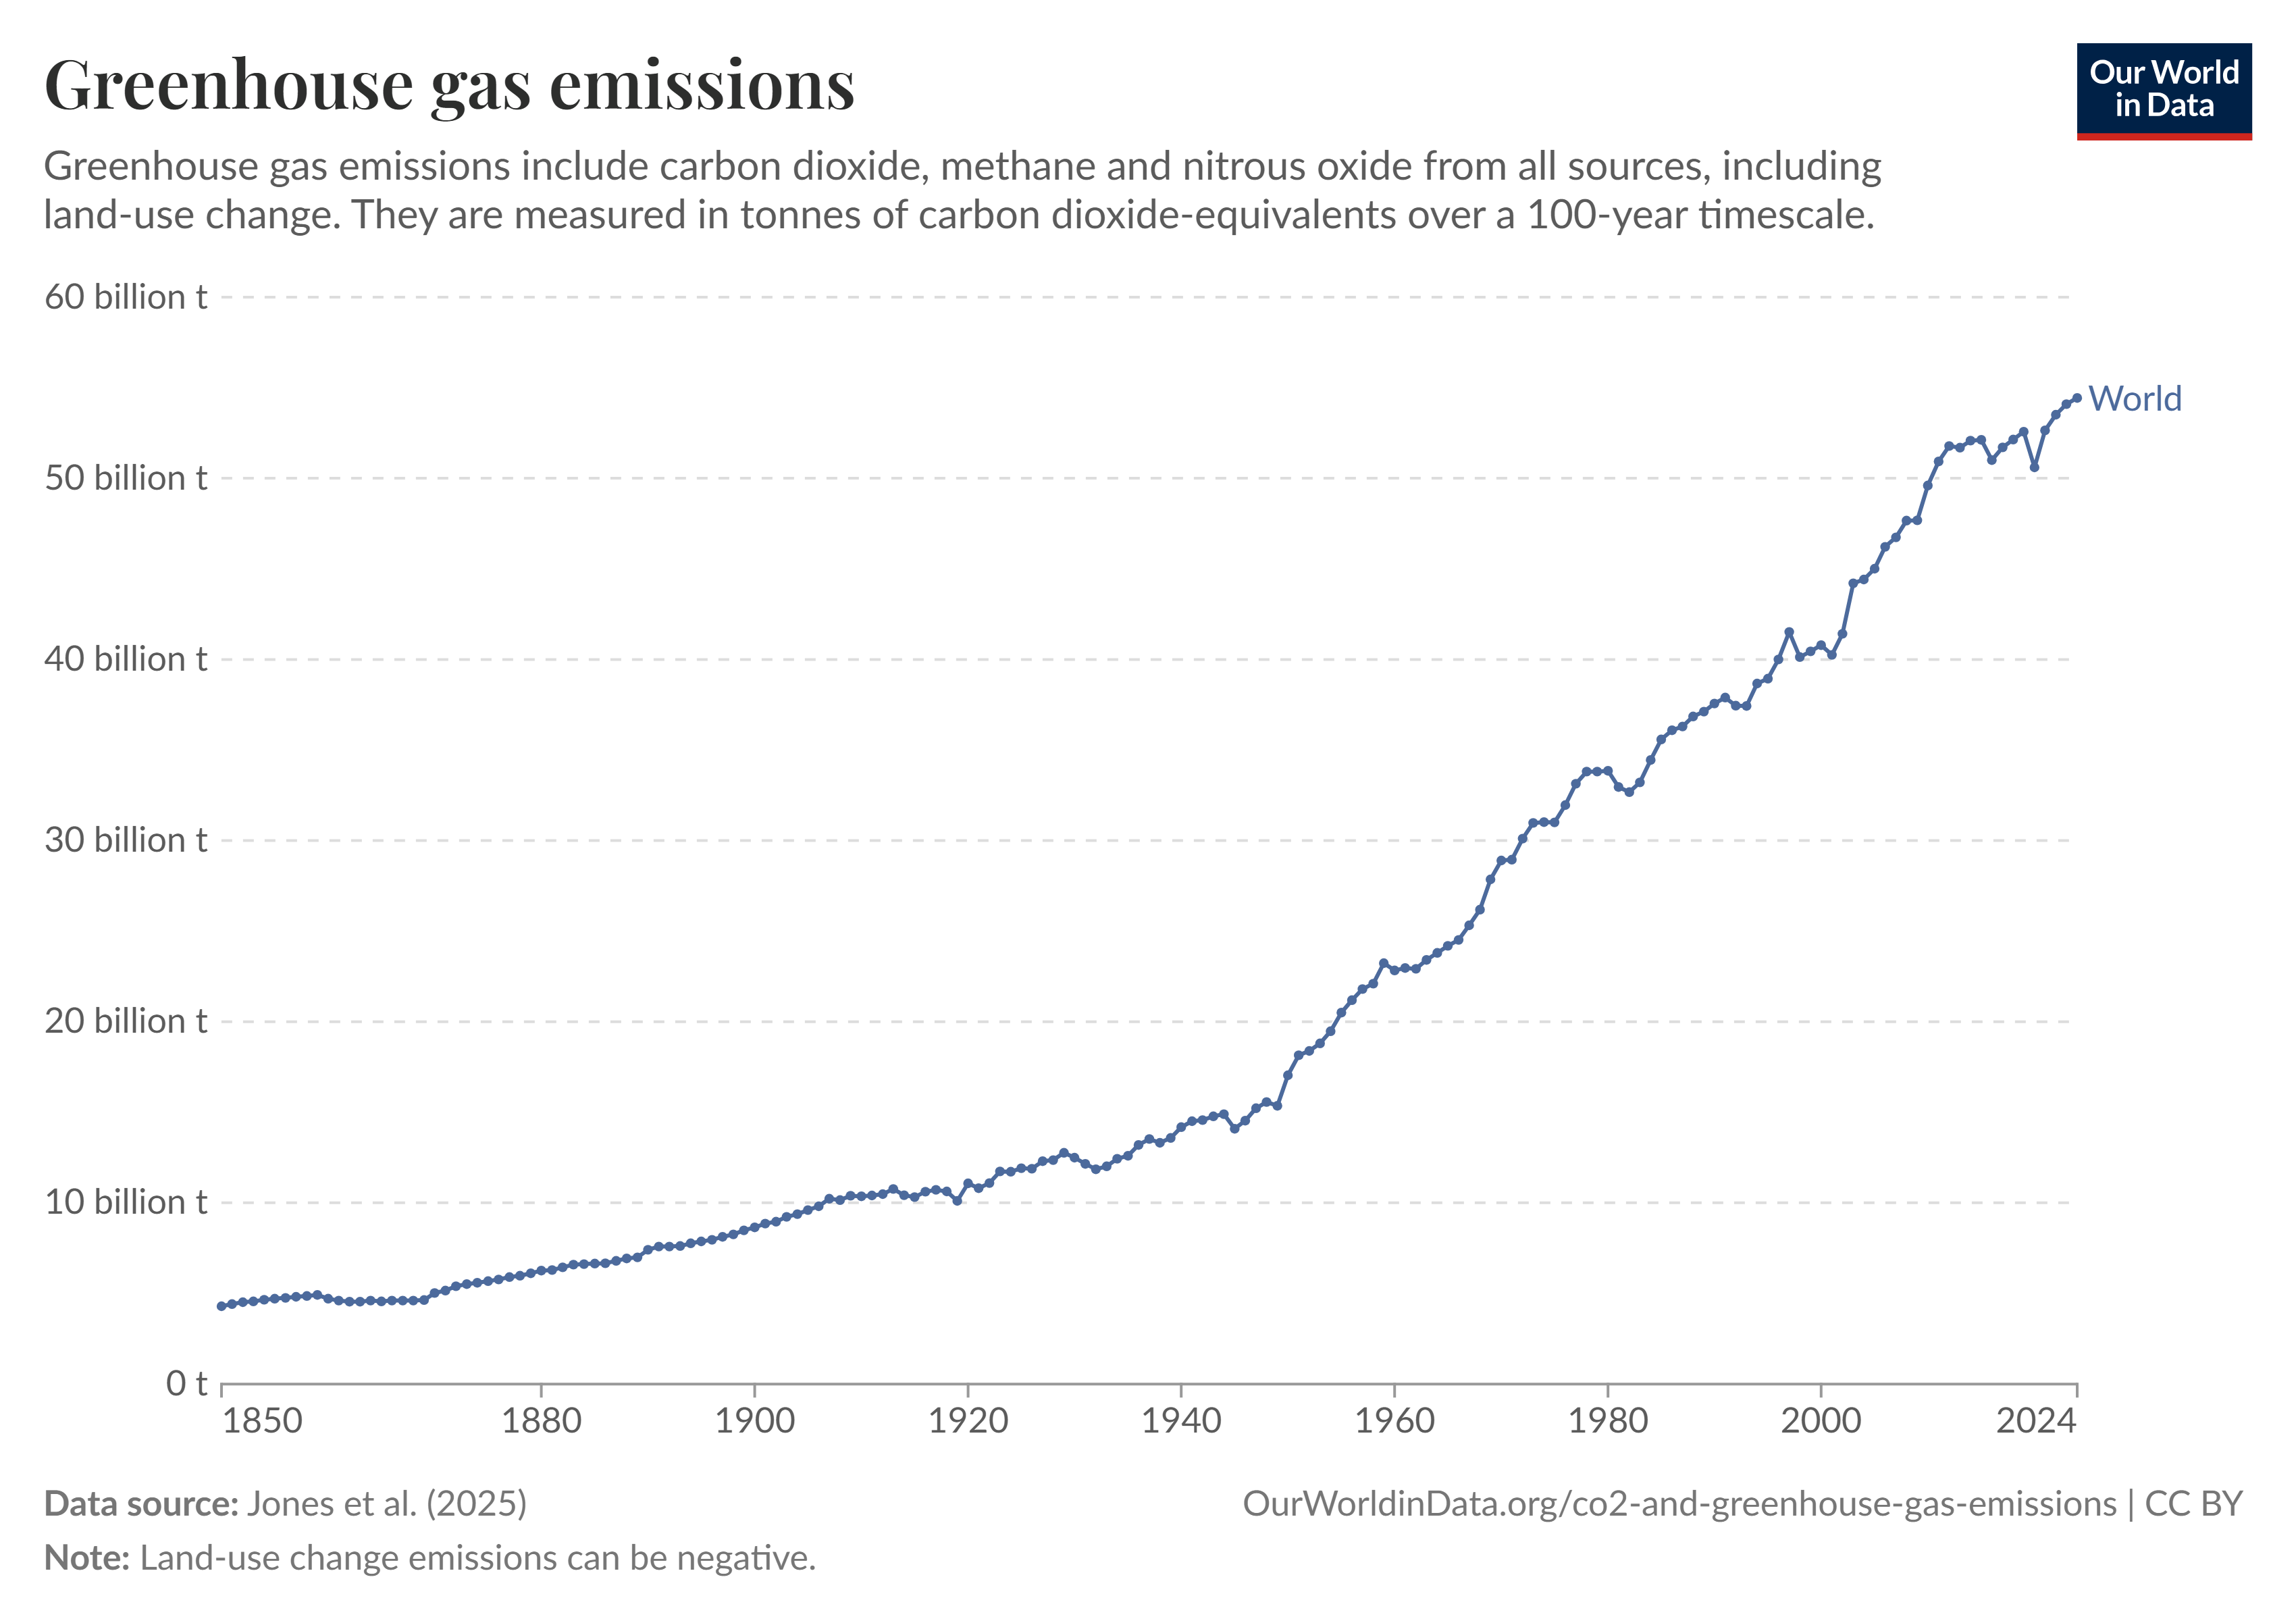
\includegraphics[width=0.9\linewidth]{Figures/greenhouse_emissions.png}
    \caption{Global greenhouse gas emissions expressed in CO\textsubscript{2}-equivalent units since 1850. Emissions include carbon dioxide, methane, and nitrous oxide from energy, industry, agriculture, and land-use change. Data source: Our World in Data, based on Jones et al. (2025) \cite{ourworldindata_ghg}.}
    \label{fig:co2}
\end{figure}

\subsection{Energy production and consumption}

The energy sector is the largest contributor to global greenhouse gas emissions. In 2018, energy related activities accounted for approximately 76\% of total global emissions when considering emissions from electricity and heat production, transport, industry, buildings, and fugitive emissions from fuel extraction and processing \cite{climatewatch_emissions}. In this section, we discuss global energy consumption, the historical composition of the global energy mix, and prospects for future energy demand and composition.

\subsubsection{Global energy consumption}

When discussing global energy production and consumption, it is important to distinguish between primary energy and final energy. Primary energy refers to the energy content of natural resources before any conversion process takes place, such as crude oil, natural gas, coal, or renewable energy flows. Final energy represents the energy delivered to end users for services such as heating, transportation, lighting, and industrial processes. 

Primary energy consumption is therefore higher than final energy consumption because energy is lost during conversion processes, including fuel refining, thermal electricity generation, and transmission and distribution losses in energy networks \cite{IEA2023}.

The magnitude of these losses depends on the conversion technology. \SI{1}{\kilo\watt\hour} of electricity delivered to the grid typically requires approximately \SI{2}{\kilo\watt\hour} of primary energy in a modern combined cycle gas turbine plant and roughly \SI{3}{\kilo\watt\hour} in coal or nuclear thermal power plants, reflecting typical thermal conversion efficiencies in the range of 30--60\% \cite{IEA2023}.

Global primary energy consumption has risen steadily over the past decades, as illustrated in Figure~\ref{fig:primary}. While the annual growth rate declined from approximately 5–6\% during the 1960s to around 1–2\% in the 2010s, absolute global energy demand continues to increase as a consequence of population growth, economic development, and expanding industrial activity \cite{ourworldindata_energy}.

\begin{figure}[htbp]
    \centering
    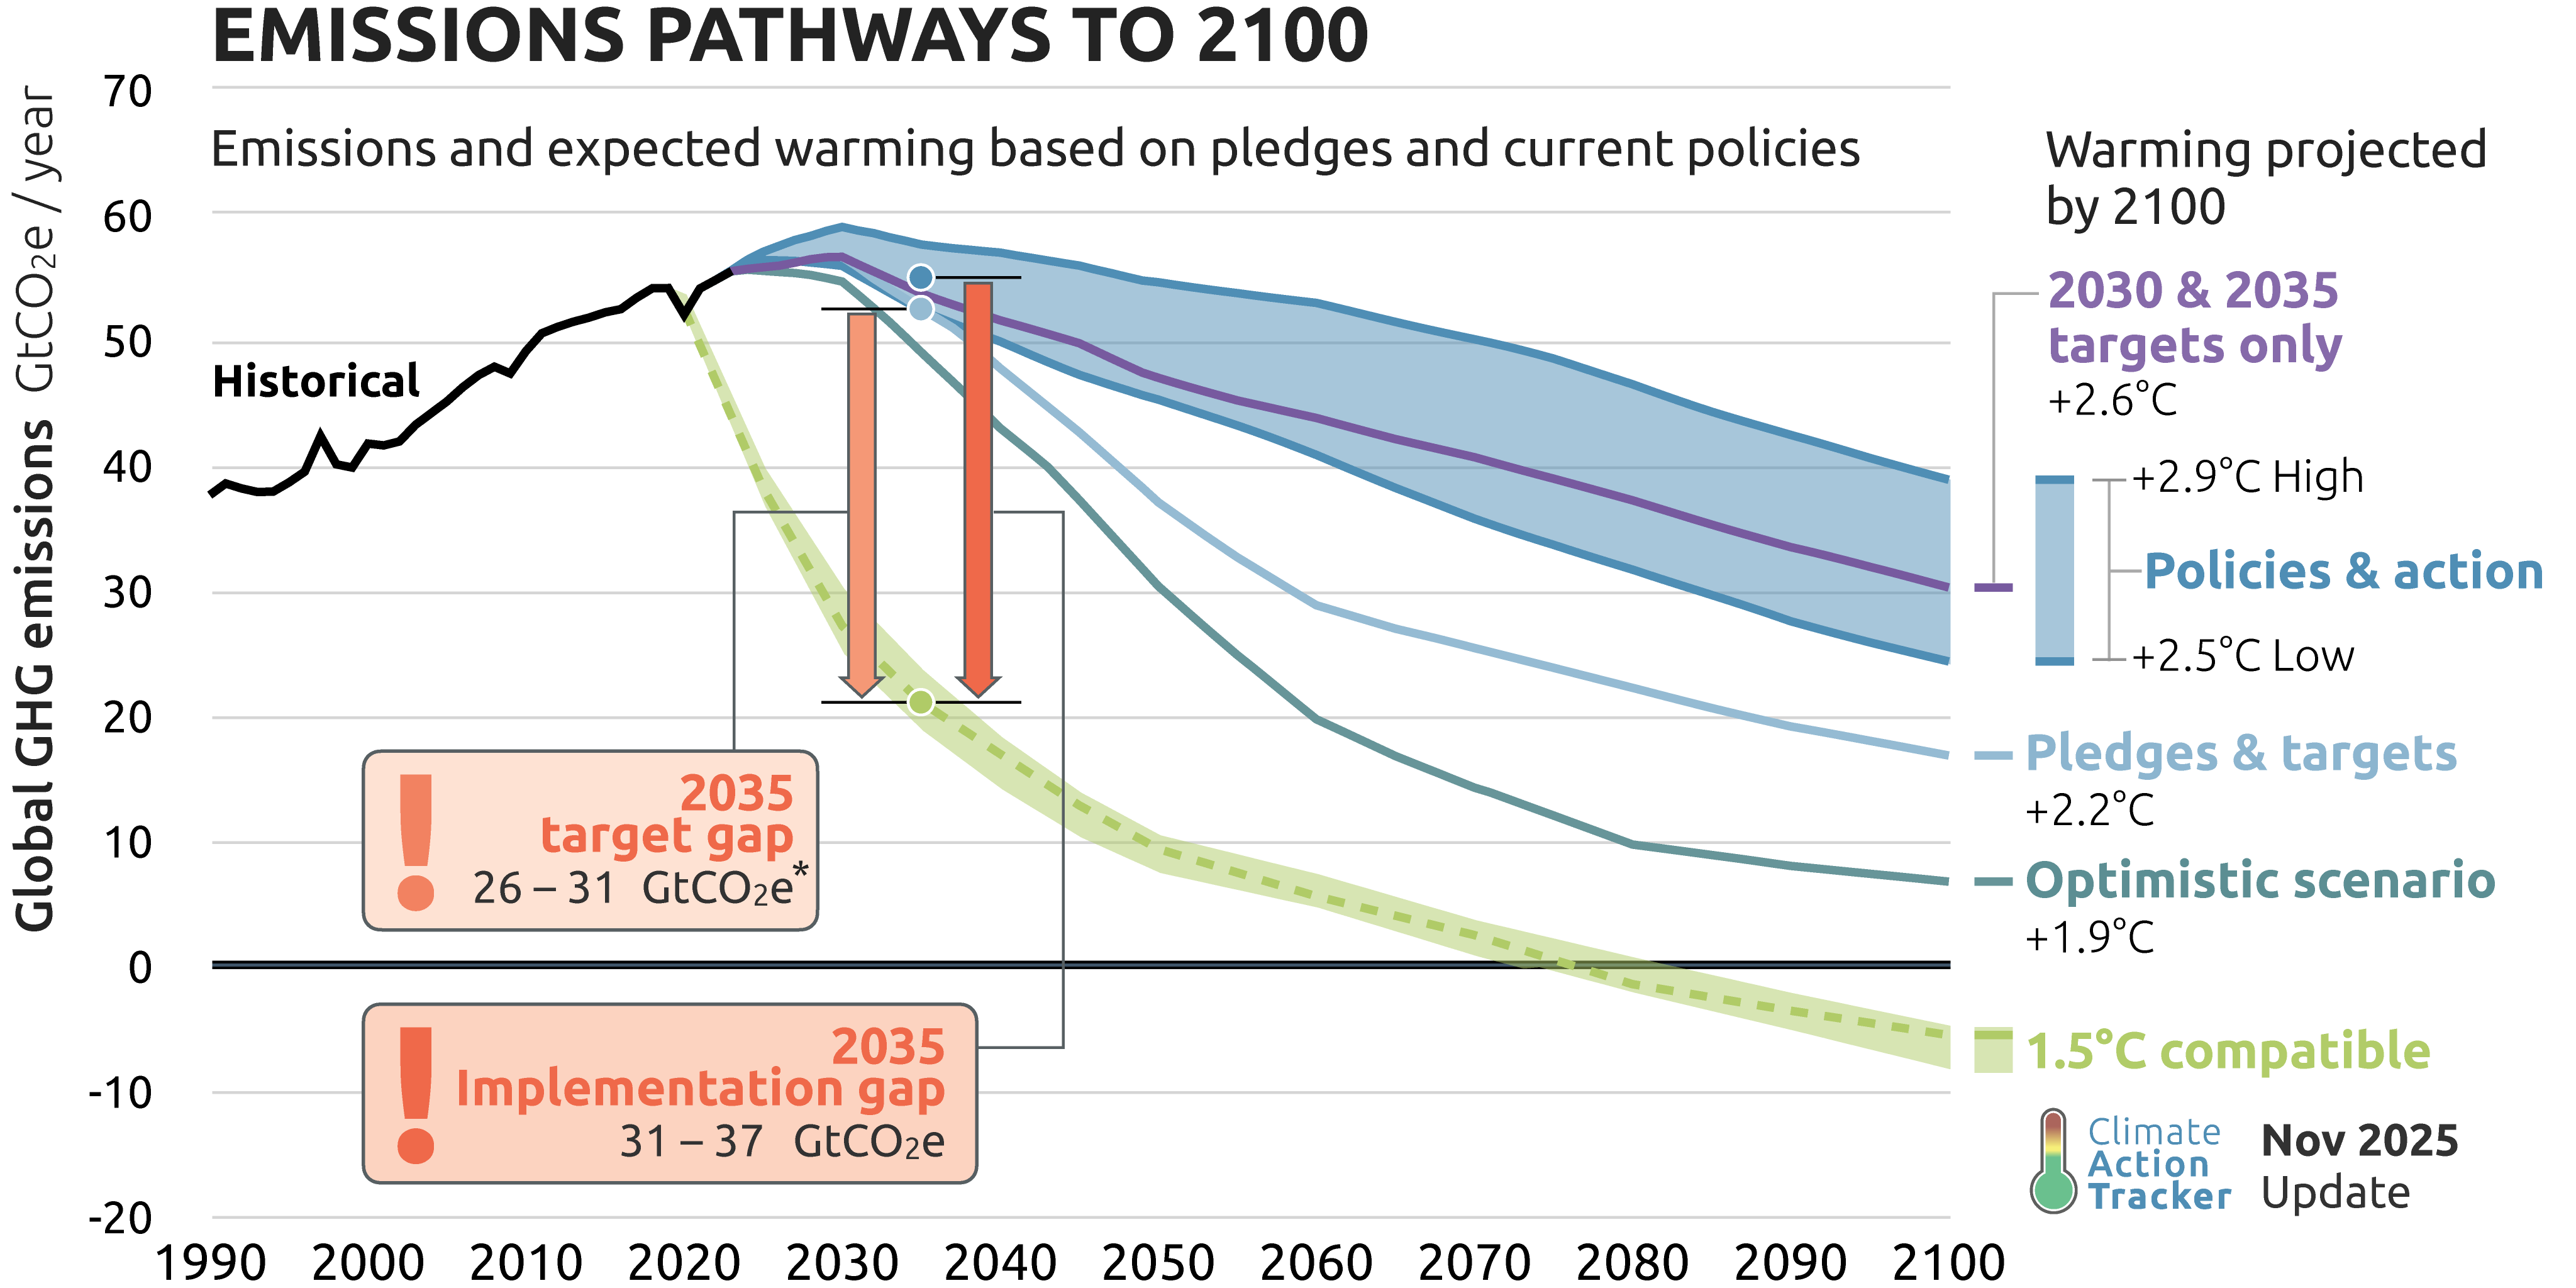
\includegraphics[width=0.9\linewidth]{Figures/emissions_path.png}
    \caption{Global greenhouse gas emission pathways under different policy scenarios and the associated projected warming outcomes by 2100. The trajectories compare current policies, pledged mitigation targets, optimistic scenarios, and pathways compatible with limiting global warming to \SI{1.5}{\celsius}. Data source: Climate Action Tracker \cite{climate_action_tracker_pathways}.}
    \label{fig:primary}
\end{figure}

In 2019, electricity accounted for approximately 19.7\% of global final energy consumption \cite{IEA2021}. More recently, the share of electricity in final energy consumption is estimated to have reached about 20\% in 2023, reflecting ongoing electrification of transportation, heating, and industrial processes \cite{iea_electricity_2024}.

\begin{figure}[htbp]
    \centering
    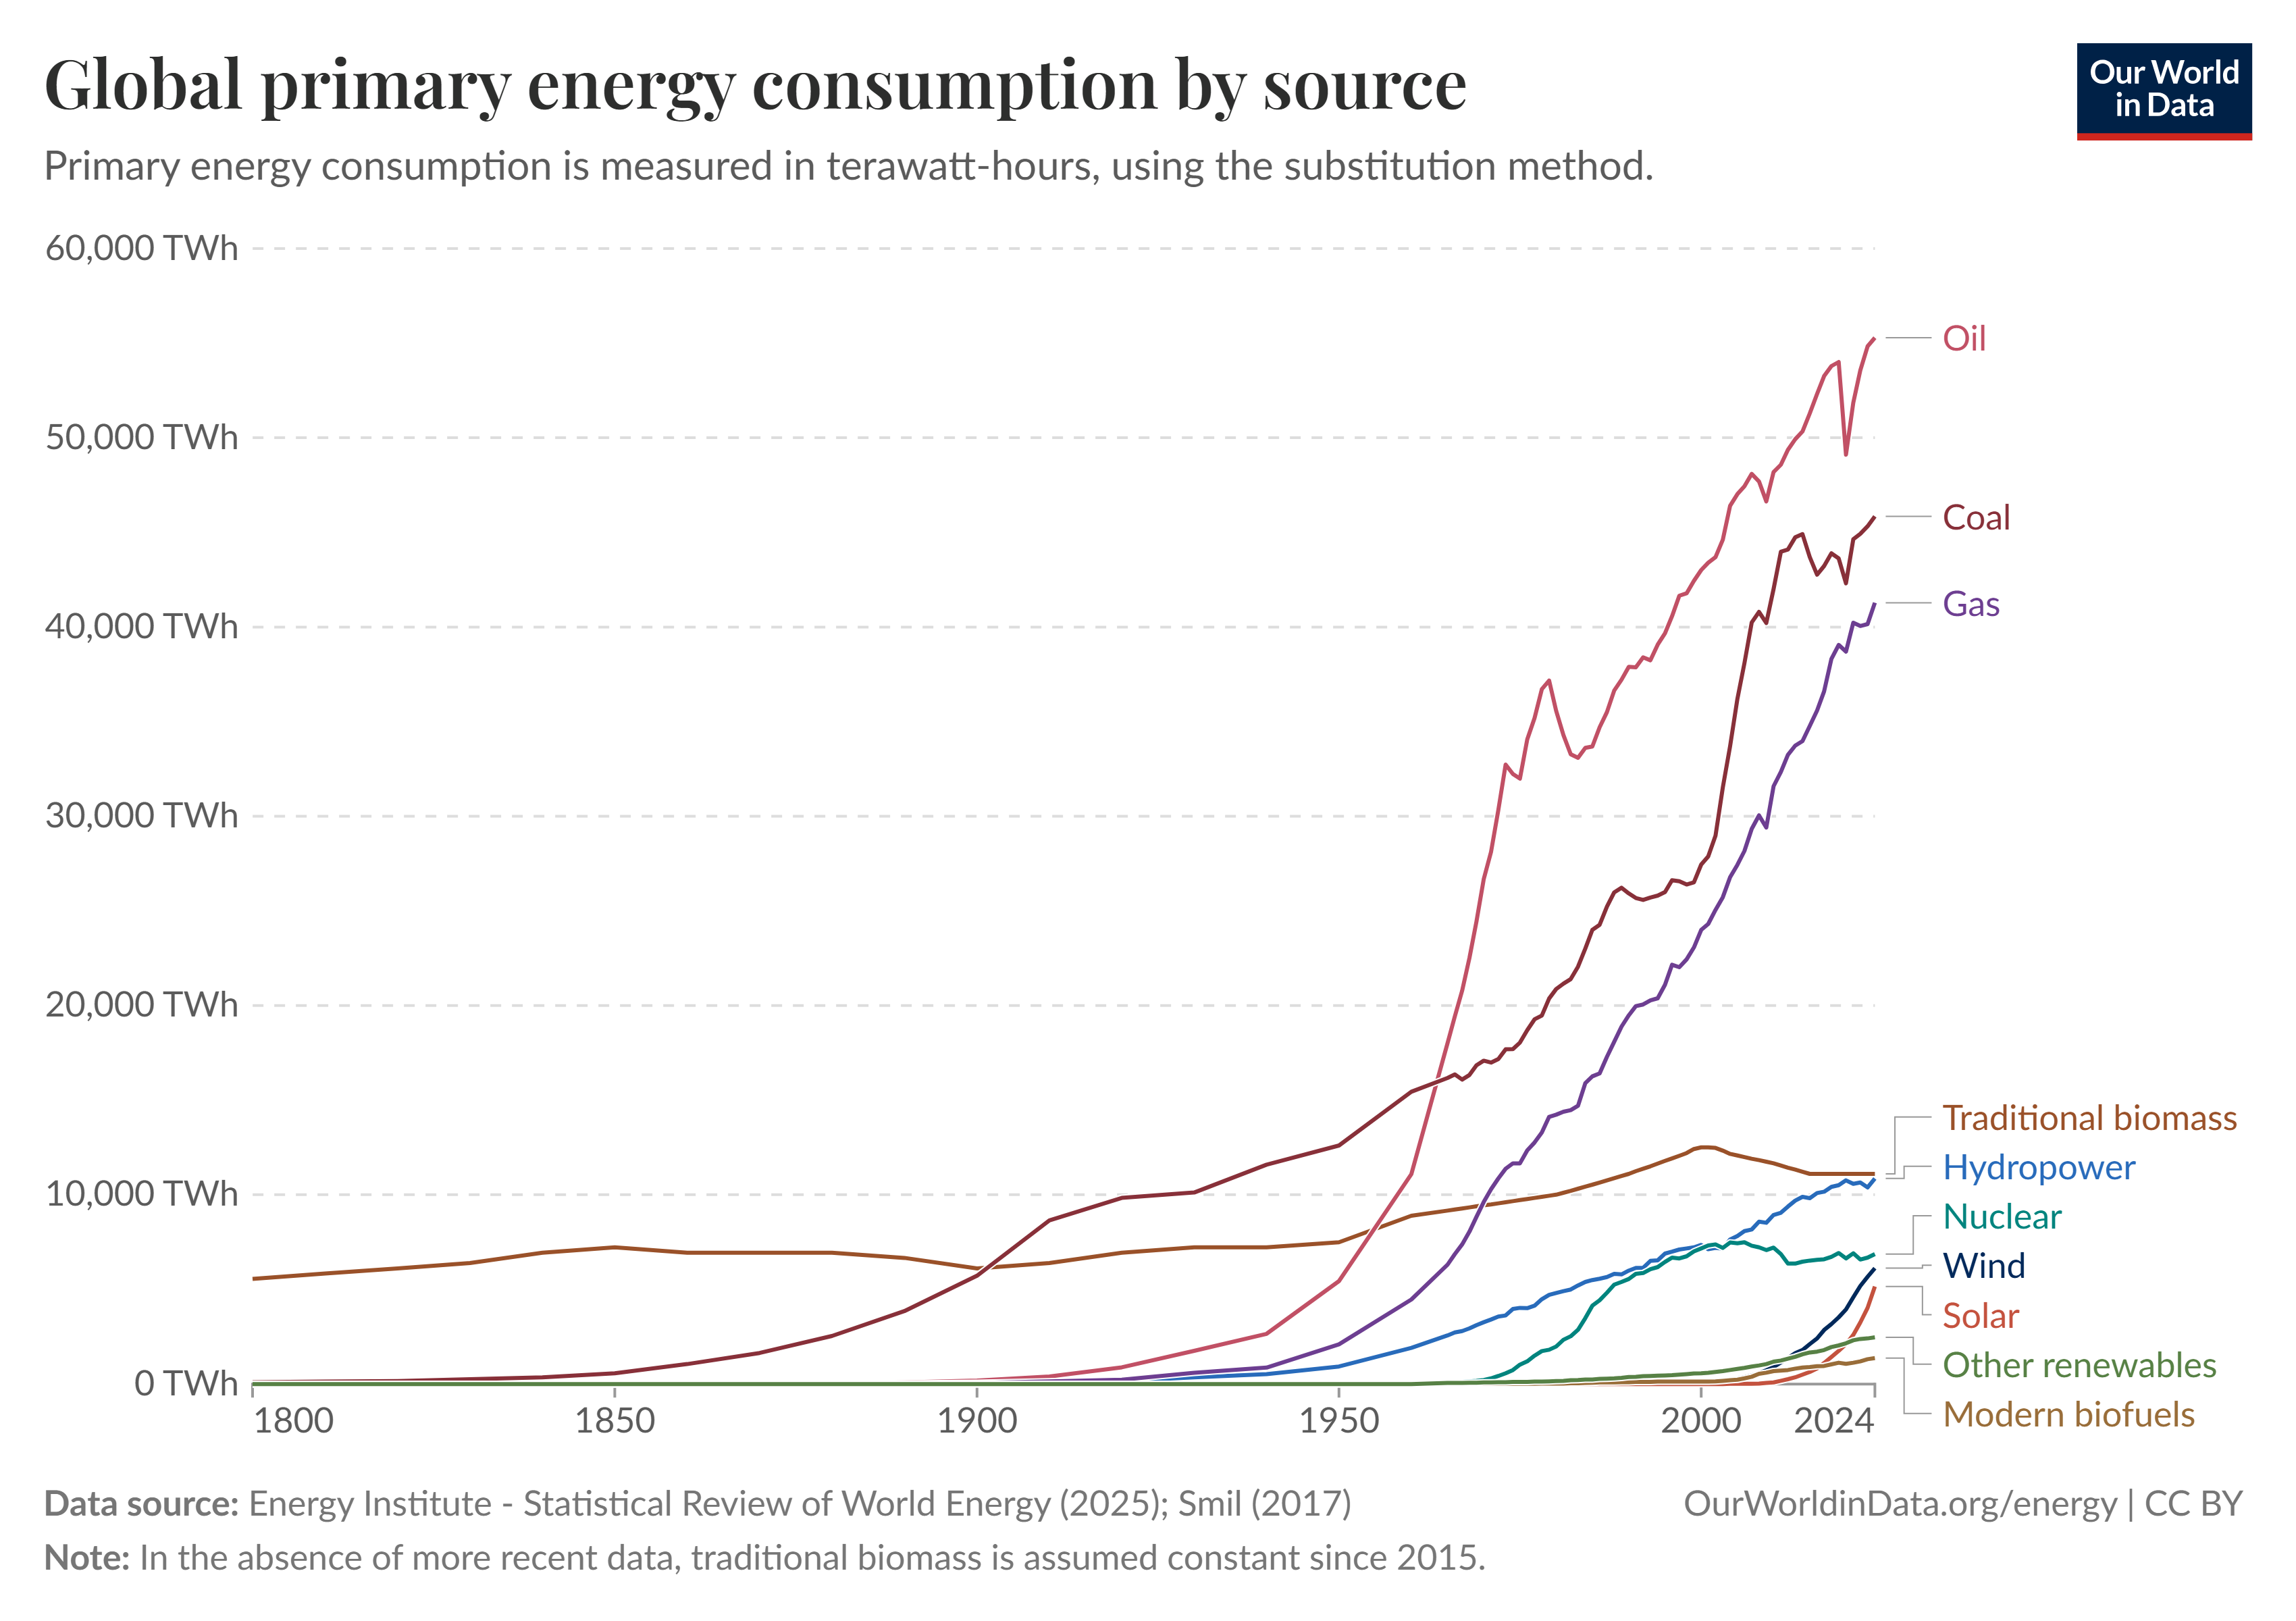
\includegraphics[width=0.9\linewidth]{Figures/global_energy_consumption.png}
    \caption{Global primary energy consumption by source since 1800. Fossil fuels continue to dominate the global energy system despite rapid growth of renewable energy technologies in recent decades. Data source: Our World in Data \cite{ourworldindata_energy}.}
    \label{fig:primary}
\end{figure}

\subsubsection{Global energy mix}
The term energy mix refers to the combination of primary energy sources used to meet energy demand. The components of the energy mix can be subdivided into fossil fuels, such as coal, oil and gas, renewable energy sources, such as hydro, wind and solar, and nuclear fission energy. Renewable energy and nuclear energy are sometimes grouped under the term low carbon energy to highlight the contrast with high carbon fossil fuel based energy.

Since the First Industrial Revolution, fossil fuels have dominated the global energy mix. The consumption of fossil fuels is still rising in absolute terms. As can be seen in Figure~\ref{fig:primary}, this is in particular due to increasing consumption of gas and, to a lesser extent, oil, while coal consumption has been closer to a plateau in global aggregate over the last decade.

Power generation through nuclear fission gained importance from the 1970s until the early 2000s, after which global generation reached a plateau. Hydropower remains the largest renewable component of global electricity generation. Wind and solar power emerged as major electricity generation technologies in the 1990s and 2000s, respectively, and their deployment expanded rapidly during the 2000s and 2010s. Other renewable energy sources include biomass and biofuels,\footnote{Biomass and biofuels are only considered renewable when the underlying biological resources are managed sustainably.} geothermal energy, waste to energy systems, and marine sources such as wave and tidal energy.
As illustrated in Figure~\ref{fig:mix2019}, although low-carbon sources accounted for only 15.7\% of total primary energy consumption in 2019, they provided approximately 36.7\% of global electricity generation. This difference reflects the fact that electricity generation can be decarbonised more readily than other sectors, such as transport and direct heat, which still rely heavily on fossil fuels.
\begin{figure}[htbp]
    \centering
    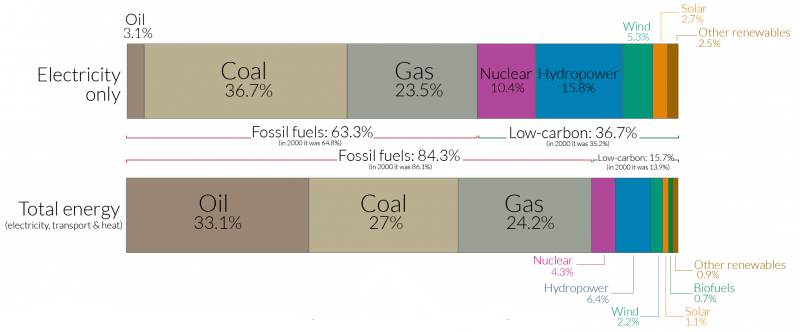
\includegraphics[width=0.9\linewidth]{Figures/Global energy mix .png}
    \caption{Global energy mix in 2019 showing the composition of electricity generation and total primary energy consumption by source. Fossil fuels dominate total energy use, while low-carbon sources represent a significantly larger share of electricity generation. Data source: Our World in Data \cite{ourworldindata_energy}.}
    \label{fig:mix2019}
\end{figure}


\subsubsection{Outlook to the future}
As Figure~\ref{fig:primary} indicates, global energy demand is continuously increasing. Between 2020 and 2100, demand is expected to more than double, driven by improvements in living standards in developing countries and by global population growth \cite{freidberg2007plasma}.

The comparison between primary energy consumption and electricity generation highlights that transitioning from fossil fuel energy to low carbon energy is generally more straightforward for applications in which electricity is the energy carrier.\footnote{Primary energy is taken based on the substitution method for energy accounting, one of the preferred accounting methods of the IPCC. It accounts for energy losses from fossil fuel conversion and provides a comparison of the low carbon energy required to replace fossil fuels in the energy mix.} Consequently, a typical strategy to decrease GHG emissions is the electrification of sectors that historically relied on fossil fuel derivatives, such as transport and heating. Crucial to the success of this strategy is the further transition from electricity generation based on fossil fuel combustion to low carbon forms of generation. Renewable energy, particularly wind and solar, is expected to play a central role in this transition. Whether the contribution of nuclear fission will increase over the coming decades remains uncertain. In Section~\ref{sec:fusion_future}, the possible role of nuclear fusion in the future energy mix is explored.

\subsection{Fusion in the energy mix of the future}
\label{sec:fusion_future}


\paragraph{Fusion vs.\ fission.}
The mass–energy equivalence 
\begin{equation}
\Delta E = \Delta m c^{2}
\end{equation}
implies that the energy released in a fusion reaction is proportional to the mass defect multiplied by the square of the speed of light. Since 
\(
c^{2} \approx 9 \times 10^{16}\,\si{m^{2}\,s^{-2}},
\)
even a minute mass defect results in a very large energy release.

The physical origin of this large energy density lies in the difference between chemical and nuclear binding. Chemical bond energies are typically on the order of electronvolts per molecule, whereas nuclear binding energies are on the order of mega–electronvolts per reaction \cite{stacey2018fusion}. As a consequence, the specific energy of fusion fuel exceeds that of fossil fuels by approximately seven orders of magnitude.

For the deuterium–tritium (D–T) reaction
\[
{}^{2}\mathrm{H} + {}^{3}\mathrm{H} \rightarrow {}^{4}\mathrm{He} + n + 17.6~\mathrm{MeV},
\]
the released energy corresponds to approximately 
\[
3.4 \times 10^{14}\,\si{J/kg}
\]
of fuel mixture under complete burn-up assumptions \cite{freidberg2007plasma}.

By comparison, the lower heating value of petrol is approximately 
\[
4.4 \times 10^{7}\,\si{J/kg}
\]
\cite{bp2023statistical}. The ratio between the two is therefore on the order of
\[
8 \times 10^{6},
\]
confirming that fusion fuel contains nearly ten million times more energy per unit mass than conventional hydrocarbon fuels.

To illustrate the scale of this difference, consider an annual electricity demand of 5\,MWh per capita for one million people, corresponding to 
\[
1.8 \times 10^{16}\,\si{J}
\]
of electrical energy \cite{iea2023electricity}.

Assuming a realistic thermal-to-electric conversion efficiency of 40\% for a fossil fuel power plant, the required primary energy would be approximately
\[
4.5 \times 10^{16}\,\si{J},
\]
corresponding to roughly
\[
10^{9}\,\si{kg},
\]
or about one million tonnes of petrol.

In contrast, assuming a net electric efficiency of 35\% for a D–T fusion power plant, the required fusion fuel mass would be
\[
\mathcal{O}(10^{2})\,\si{kg}.
\]

Thus, a few hundred kilograms of fusion fuel could provide the same annual electricity supply as approximately one million tonnes of fossil fuel.


\paragraph{Fusion vs.\ fossil fuels.}

Beyond the comparison with fission, fusion must also be evaluated against conventional fossil fuel power generation, which currently dominates global electricity production. A fundamental distinction arises from the specific energy density of the fuel. Combustion processes release energy through chemical bond rearrangement, with typical energy densities on the order of $10^{7}\,\si{J/kg}$ for hydrocarbon fuels \cite{bp2023statistical}. In contrast, the deuterium--tritium fusion reaction releases approximately $3.4 \times 10^{14}\,\si{J/kg}$ under complete burn-up assumptions \cite{stacey2018fusion}. The resulting difference of nearly seven orders of magnitude implies that the mass of fuel required for fusion power production is negligible compared with that required for fossil fuel generation.

This difference has systemic implications. Fossil fuel power plants rely on continuous extraction, transport, storage, and combustion of large volumes of fuel, introducing supply chain dependencies and exposure to geopolitical risks. Fusion, by contrast, relies primarily on deuterium extracted from seawater and lithium for tritium breeding, both widely distributed resources. From an energy security perspective, this reduces dependence on geographically concentrated fuel reserves and mitigates exposure to fuel price volatility.

Environmental impact further differentiates the two systems. Fossil fuel combustion emits significant quantities of carbon dioxide, contributing directly to anthropogenic climate change \cite{ipcc_ar6_syr_2023}. Fusion reactions themselves produce no greenhouse gases during operation. Although lifecycle emissions arise from construction, materials production, and plant decommissioning, the operational phase is effectively carbon free.

The economic structure of the two technologies also differs significantly. Fossil fuel power plants typically exhibit cost structures in which fuel represents a substantial fraction of the levelized cost of electricity (LCOE), particularly for gas-fired generation \cite{iea_electricity_2024}. In fusion systems, by contrast, fuel costs are negligible relative to capital expenditure and operations and maintenance. Consequently, the economic competitiveness of fusion is expected to depend primarily on plant availability, reliability, and component lifetime rather than on fuel market dynamics. This shifts the optimisation focus from fuel procurement toward asset performance and long-term system reliability.


\paragraph{Fusion vs.\ renewables.}

Fusion must also be evaluated relative to renewable energy technologies such as wind and solar photovoltaics, which are currently expanding rapidly and exhibit sharply declining levelized cost of electricity (LCOE) \cite{IEA2023}. Unlike fossil fuels, renewables provide low-carbon electricity during operation and therefore compete directly with fusion in the context of decarbonized energy systems.

The primary distinction lies in energy density and dispatchability. Wind and solar energy sources are inherently intermittent, with capacity factors typically ranging between 20--35\% for solar and 30--50\% for onshore wind depending on location \cite{IEA2023}. Their output depends on meteorological conditions and diurnal cycles. Fusion power plants, similar to fission plants, are designed for high capacity factor baseload operation, with projected values above 70--80\% in techno-economic studies \cite{Lindley2023}. This distinction implies fundamentally different roles within the energy system.

Because renewable output is variable, large-scale integration requires grid flexibility, storage, or overcapacity to ensure supply--demand balance. Storage technologies, including batteries and hydrogen, introduce additional capital costs and system-level efficiency losses. Fusion, by contrast, produces controllable thermal power and can provide firm generation without reliance on weather conditions. In long-term decarbonization scenarios, system modelling studies suggest that firm low-carbon sources can reduce total system cost when renewable penetration becomes very high \cite{Lindley2023}.

Land use intensity also differs significantly. Solar and wind installations require substantial spatial deployment due to their lower areal power density. Fusion, similar to fission, concentrates large power output within a comparatively small footprint. This may become relevant in regions with limited available land or high population density.

Economically, renewables benefit from short construction times and modular scalability, whereas fusion plants are capital-intensive infrastructure projects with longer development timelines. However, once operational, fusion plants are expected to exhibit low marginal operating costs and stable output. The competition between fusion and renewables therefore depends not only on plant-level LCOE but also on system-level integration costs, reliability requirements, and decarbonization targets.

Rather than representing mutually exclusive pathways, fusion and renewables may be complementary in a deeply decarbonized electricity system: renewables providing low-cost variable generation, and fusion offering firm, dispatchable, high-density power that stabilizes the grid and reduces the need for large-scale storage.

\subsubsection{Recent developments in fusion}
\label{sec:recent_fusion}

Research into controlled thermonuclear fusion for power generation has been ongoing since the 1940s. However, the global fusion landscape has recently entered a qualitatively different phase, characterised not only by scientific progress but also by simultaneous developments in publicly funded flagship programmes, rapid expansion of private sector initiatives, and increasing engagement by regulators, investors, utilities, and industrial supply chains.

According to the \textit{IAEA World Fusion Outlook 2025}, nearly 40 countries operate active fusion programmes, global private investment has surpassed US\$10~billion, and more than 160 fusion devices are operational, under construction, or planned~\cite{iaea_wfo_2025}. These developments indicate a gradual transition from purely experimental research facilities toward early industrialisation pathways. In this context, plasma physics achievements increasingly intersect with deployment requirements such as licensing frameworks, supply chain qualification, capital investment, and long term asset reliability.

Magnetic confinement fusion (MCF), discussed in Section~\ref{sec:Eng_fusion}, aims to achieve fusion conditions by confining a high temperature plasma using magnetic fields. The most advanced MCF concepts are tokamaks and stellarators, which provide toroidal magnetic confinement, although alternative configurations have also been investigated.

The most prominent experimental device to date has been the Joint European Torus (JET), which achieved a fusion gain of \(Q = 0.67\), producing 16~MW of fusion power from 24~MW of external heating power. During its final deuterium--tritium campaign, JET produced a total fusion energy of 69.26~MJ in a single pulse lasting approximately six seconds~\cite{eurofusion_jet_record_2024}. 

Although these experiments did not achieve net electricity production, they provided critical validation of plasma physics models, auxiliary heating systems, and tritium fuel cycle operation. These results constitute a key experimental foundation for next generation devices such as ITER and DEMO.

Progress has also been achieved in long pulse plasma operation. The EAST tokamak sustained plasma operation at approximately 70~million~°C for 1066~s following upgrades to heating systems and diagnostics~\cite{iaea_wfo_2025}. Such long duration discharges are particularly relevant for steady state reactor scenarios, where component fatigue, material degradation, and plasma control stability become critical constraints.

A major milestone in large scale fusion infrastructure is the ongoing construction of the ITER tokamak. ITER is designed to produce 500~MW of fusion thermal power for 50~MW of external heating over pulses lasting several hundred seconds. The project represents one of the most complex scientific collaborations ever undertaken and involves the integration of superconducting magnets, cryogenic systems, tritium handling facilities, and remote maintenance technologies. ITER therefore serves not only as a physics experiment but also as a large scale demonstration of the engineering and industrial capabilities required for future fusion power plants.

In parallel with publicly funded programmes, private sector activity has expanded rapidly over the past decade. More than 40 private fusion companies are currently pursuing diverse technical approaches, including compact high field tokamaks, stellarators, magnetised target fusion, and inertial confinement concepts. Several firms have raised funding rounds exceeding hundreds of millions of US dollars, and cumulative private investment has reached multi billion dollar levels~\cite{fusion_industry_association_2024}.

\begin{figure}[htbp]
    \centering
    
    % --- Main image (Figure 4) ---
    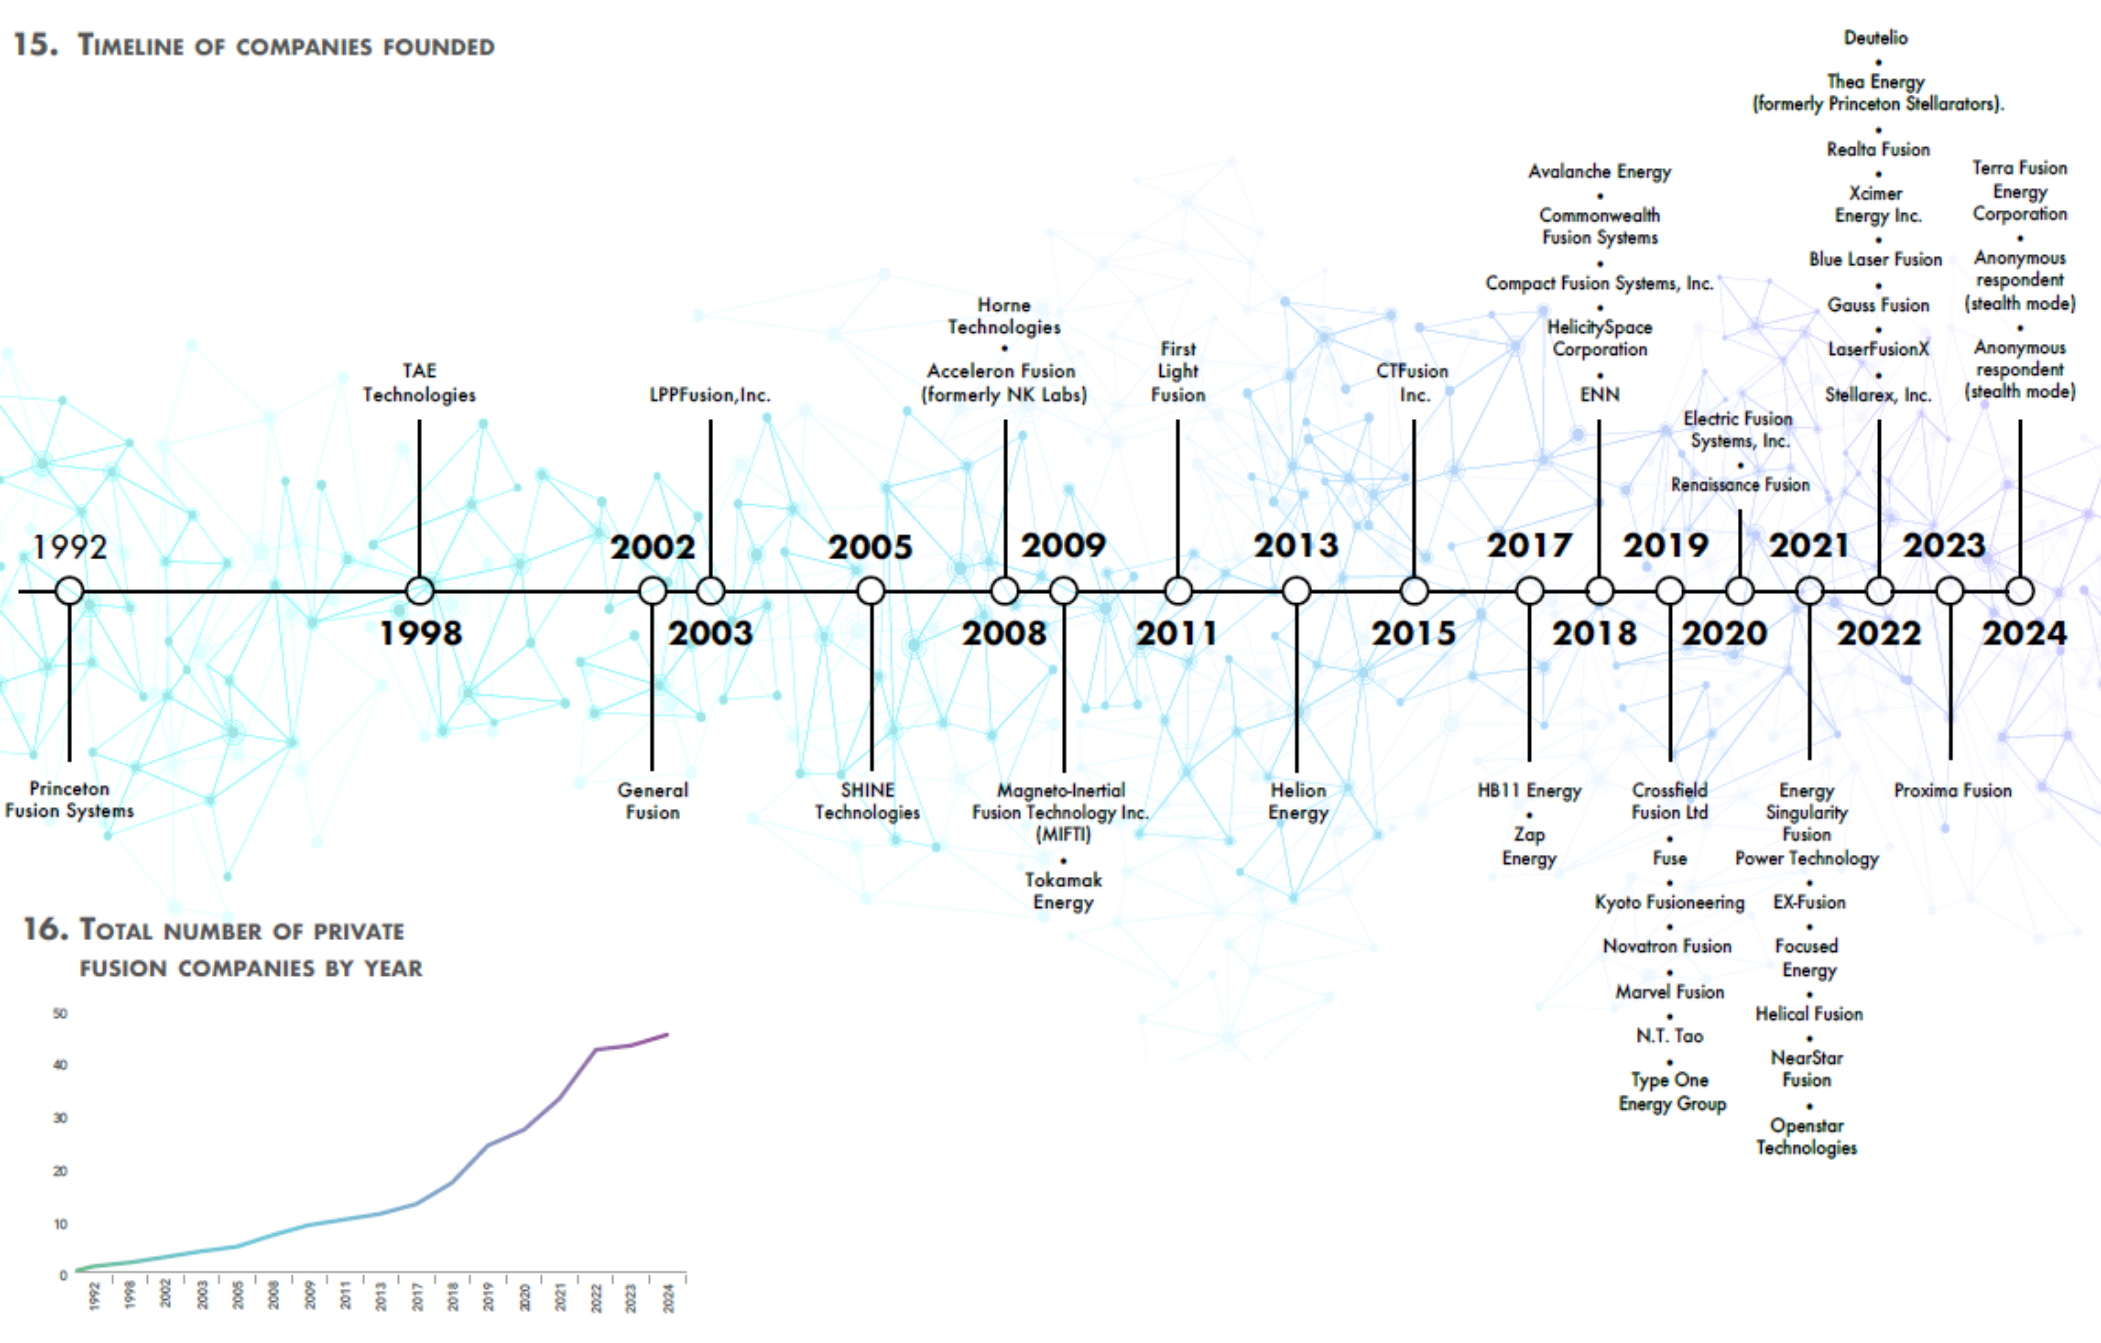
\includegraphics[width=0.9\textwidth]{Figures/companies_founded.png}
    
    \vspace{0.5cm}
    
    % --- Smaller image underneath (Figure 5) ---
    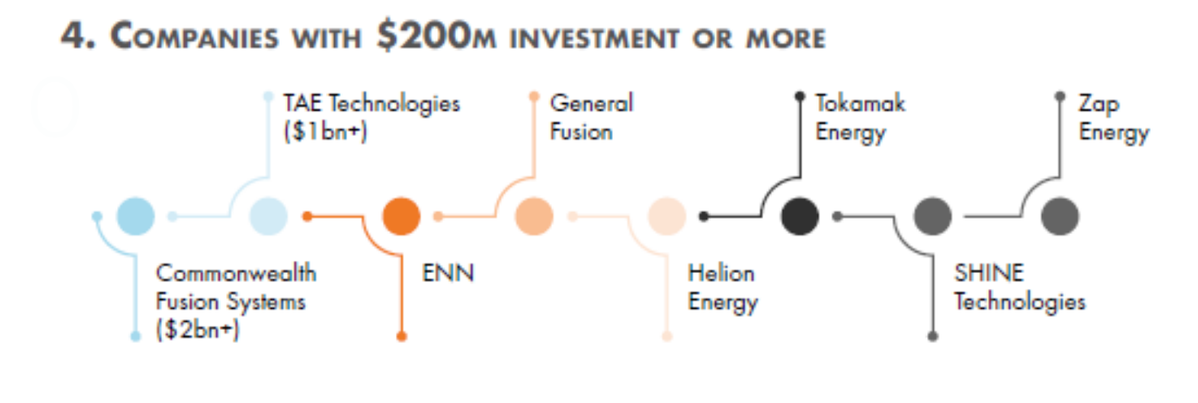
\includegraphics[width=0.55\textwidth]{Figures/companies_investment.png}
    
    \caption{
    Overview of private fusion industry development. 
    \textbf{Top:} Timeline of private fusion companies and growth in the number of active companies. 
    \textbf{Bottom:} Major private fusion companies with investments exceeding \$200 million.
    }
    
    \label{fig:fusion_private_industry}
\end{figure}

Recent developments include demonstrations of high temperature superconducting magnets enabling higher magnetic field strengths in compact devices, announcements of pilot plants targeting grid connection in the 2030s, and early agreements with utilities and industrial partners exploring future power purchase arrangements. While these initiatives remain at a pre commercial stage, they indicate that fusion is increasingly evaluated within an industrial and market context rather than solely as a long term research objective.

Another pathway to fusion is inertial confinement fusion (ICF), also discussed in Section~\ref{sec:Eng_fusion}. In December 2022, the National Ignition Facility achieved laser driven fusion ignition, producing 3.15~MJ of fusion energy from 2.05~MJ of laser energy delivered to the target~\cite{llnl_nif_ignition_2022}. Subsequent experiments have reproduced ignition conditions under controlled configurations. Although this represents a major physics breakthrough, practical energy applications would require orders of magnitude improvements in repetition rate, driver efficiency, target fabrication cost, and overall system integration.

Across both MCF and ICF pathways, regulatory and industrial considerations are gaining increasing attention. Several countries are currently developing regulatory frameworks specifically adapted to fusion technologies, distinct from traditional fission licensing regimes. At the same time, industrialisation challenges are becoming more visible, including supply chain constraints for superconducting materials, specialised manufacturing capabilities, and the development of a skilled workforce.

These developments are particularly relevant for DEMO and subsequent first of a kind reactors. Whereas ITER aims to demonstrate high fusion gain and plasma performance, DEMO must demonstrate net electricity production, a closed tritium fuel cycle, remote maintainability under reactor relevant neutron loads, and sustained high plant availability. In this context, plant economics become strongly dependent on operational reliability. Given the capital intensive nature of fusion facilities, reductions in plant availability can significantly affect the Levelized Cost of Electricity. Consequently, advanced diagnostics, monitoring, and predictive maintenance strategies become structural design requirements for commercial fusion power plants rather than secondary optimisation tools.

Recent international assessments of the fusion sector identify several key challenges that must be addressed for the transition from experimental devices to commercial power plants. These include achieving reliable and sustained plasma performance, qualification of materials under reactor relevant neutron loads, development of a closed tritium fuel cycle, integration of complex subsystems at reactor scale, establishment of regulatory and licensing frameworks, and maturation of industrial supply chains and manufacturing capabilities~\cite{iaea_wfo_2025,fusion_industry_association_2024}.

\begin{comment}
\section{The Joint European Torus (JET)}
\label{sec:JET}
The Joint European Torus (JET), based at the Culham Centre for Fusion Energy, UK, is one
of the main research facilities of the European fusion programme, and, as such, one of the
largest collaborative experiments worldwide. JET has been in operation since 1983, and was explicitly
designed to study the behaviour of plasmas in conditions and dimensions approaching those
required in a (commercial) fusion reactor. When it was built, the hope was to eventually reach
breakeven operation. JET did not achieve this, but it is to date the record holder among all
magnetic confinement fusion devices, with an energy efficiency of 67\%~[31]. Today, after having
undergone multiple transformations to become more ITER-like, its primary task is to prepare
for the construction and operation of ITER~[21].

In this chapter, the main principles of the design of JET are developed from the principles
of magnetic confinement fusion. Furthermore, the main mechanisms for plasma heating are
discussed.

\subsection{Machine design}
In this section, the principles of magnetic confinement are explored in more detail. Then,
the tokamak configuration is introduced, explaining how magnetic confinement is realised for
nuclear fusion devices such as JET. Finally, some components in the chamber design of JET are
discussed, including the materials its components are made of.

\subsection*{Magnetic confinement}
In \ref{sec:Eng_fusion}, the magnetic confinement scheme was briefly touched upon. In this confinement
scheme, magnetic fields are used to confine the fusion fuel. This is possible as the fusion fuel is
at such high temperature that all particles are completely ionized, yielding a highly conductive
medium, the plasma.

To understand the working of magnetic confinement, consider a cylinder containing plasma par-
ticles. Without an externally applied magnetic field, the motion of the individual plasma particles
is seemingly random. Plasma particles collide with each other and with the cylinder’s
boundaries, the collision frequency being dependent on the kinetic energy of the particles.

If now an external magnetic field is applied parallel to the cylinder’s central axis, the magnetic
force component of Lorentz’s law, expressed by Equation~\eqref{eq:lorentz}, will affect the path of the charged
particles. In this equation, \(q\), \(\vec{v}\), \(\vec{E}\) and \(\vec{B}\) denote the charge of the particle, the particle velocity,
the electric field and the magnetic field:
\begin{equation}
\vec{F} = q\,(\vec{E} + \vec{v} \times \vec{B}).
\label{eq:lorentz}
\end{equation}

From Equation~\eqref{eq:lorentz} it can be derived that the path of the charged particles will now be helical
around the magnetic field lines, referred to as the \emph{guiding centre path}. The guiding centres
move parallel to the applied field, with particles of opposite charges rotating around the
central axis in opposite directions. The path of the particles without any external fields and
with an external magnetic field can be seen in Figure~\ref{fig:helixmotion}.

\begin{figure}[h]
  \centering
  \fbox{\rule{0pt}{60mm}\rule{0.95\linewidth}{0pt}}
  \caption{Motion of charged particles without (left) and with (right) an external magnetic field. [TO CHECK: original source]}
  \label{fig:helixmotion}
\end{figure}

The helical motion prevents the particles from collisions with the wall, whereas collisions with
other particles, possibly resulting in fusion reactions, are still possible.

As Figure~\ref{fig:helixmotion} illustrates, the ideal shape for a fusion vessel would be an infinite cylindrical tube.
Two possible configurations that approximate this infinite tube are depicted in Figure~\ref{fig:mirror-torus}~[5].

\begin{figure}[h]
  \centering
  \fbox{\rule{0pt}{58mm}\rule{0.95\linewidth}{0pt}}
  \caption{Magnetic confinement configurations: mirror confinement (left) and torus confinement (right)~[5].}
  \label{fig:mirror-torus}
\end{figure}

In the mirror confinement configuration, the magnetic fields at the end points are stronger.
Consequently, some particles will be mirrored whereas others will escape the vessel. In the torus
confinement configuration, end-point losses are prevented altogether.



\subsection*{Tokamak configuration}
JET uses the torus confinement configuration. To create the magnetic field, different machine
configurations are possible. In JET, the tokamak configuration is used. A schematic representa-
tion of the elements of a tokamak, as well as the layout of JET, are given in Figure~\ref{fig:tokamak-jet}.

\begin{figure}[h]
  \centering
  \fbox{\rule{0pt}{58mm}\rule{0.95\linewidth}{0pt}}
  \caption{Schematic representation of a tokamak (left) and layout of JET (right)~[32].}
  \label{fig:tokamak-jet}
\end{figure}

The almost torus-shaped plasma container of the JET fusion device is ringed by thirty-two
D-shaped toroidal field coils. The D-shape is preferred over a circular shape as the stress on
the coils, caused by the bending of the coils, is reduced due to the D-shape. Each coil consists
of twenty-four individual coils, each carrying a current of up to \SI{80}{\kilo\ampere}, adding up to a total
magnetic field of maximum \SI{4}{\tesla}. For more modern tokamak designs, superconducting coils are
to be preferred over copper coils, given their near-zero resistivity~[21].

The torus confinement configuration ensures that no particles leak through the end point of the
plasma vessel. This configuration does, however, introduce new leakage problems. As in a torus
configuration, the distance between coils at the centre differs from the distance between coils
near the outer wall, the magnitude of the magnetic field is bigger at the centre, and the plasma
drifts outwards.

To counter the outward plasma drift, poloidal field coils are introduced on the in- and outside of
the torus, together inducing a poloidal magnetic field. The inner coils generate a large poloidal
magnetic field, which generates a large toroidal plasma current, similar to a transformer’s op-
eration. The plasma current enhances the poloidal field, thereby creating an inward force and
having a pinching effect on the plasma itself. In order to control the stability of the relatively
unstable current-driven plasma, outer poloidal field coils are added.

The combination of the poloidal field with the toroidal field yields a helical magnetic field that
continuously drives particles from the weaker outer field to the stronger inner field, and vice
versa. This has a stabilizing effect on the plasma. For completeness, we mention that various
other approaches for creating a helical magnetic field exist. The most important example so far is
the stellarator reactor design, in which the helical field is produced using a complex arrangement
of magnets~[5].

\subsection*{Chamber design}
The machine vessel, containing a \SI{150}{\mega\kelvin} plasma, has to sustain the immense loads
generated by it, making the design of such a vessel a very challenging task. In Figure~\ref{fig:jet-chamber},
the JET plasma chamber, along with its main components and the materials of which they are made, is
shown.

\begin{figure}[h]
  \centering
  \fbox{\rule{0pt}{58mm}\rule{0.95\linewidth}{0pt}}
  \caption{JET plasma chamber~[33].}
  \label{fig:jet-chamber}
\end{figure}

\paragraph{Limiters.}
Even with the helical magnetic field configuration of the tokamak, plasma leakages are inevitable.
Upon collision with device components, plasma particles will cause erosion. The eroded particles
will contaminate and cool down the plasma, eventually quenching it. For this reason, beryllium
(Be) limiters are placed at the inner and outer edges of the plasma. The limiters prevent the
outward-going ions from colliding with the wall. Consequently, the ions are eroding the limiters
rather than other plasma-facing components (PFCs). As Be is a light atomic element, plasma
contaminated with Be particles experiences lower Bremsstrahlung losses compared to plasma
contaminated with heavier particles, making Be the best material choice for the limiters~[34].

\paragraph{Divertor.}
Even if tungsten (W) is more erosion-resistant, some erosion will still take place. For this reason,
a divertor is installed at the bottom of the vessel. By tuning the magnetic field, most eroded ions are
diverted from the plasma to the divertor. Hence, the divertor acts as an exhaust for power and
for the particles crossing the outermost closed magnetic flux surface.

Helium, the reaction product of the fusion reaction, dilutes the fuel after its kinetic energy has
been re-invested into the plasma. The second reason for the installation of the divertor is the
extraction of the helium from the plasma~[34].

\paragraph{First wall.}
The first fusion product, helium, is extracted via the divertor. The second fusion product, the
neutrons, however, are not affected by magnetic fields, and thus collide with the walls of the
vessel, where they will cause erosion. As this erosion is unavoidable, it is best to choose a
material that will contaminate the plasma the least. The low-Z material beryllium (Be) is a
good candidate, as low-Z impurities are more easily ionized in a plasma. Consequently, they will
drift to the outermost closed magnetic flux surface more swiftly, from where they are diverted
towards the divertor and out of the plasma. Additional benefits of Be are its high thermal
conductivity and the fact that it reflects neutrons well.

The first wall, which is similar to the first wall that will be used in ITER, consists of a Be-
coated material that is segmented into tiles to reduce eddy currents, which are currents that
flow in closed loops within conductors, in planes orthogonal to the magnetic field. The neutrons
colliding with the wall are highly energetic and thus produce a lot of heat upon collision. Future
devices could make use of turbines to convert the produced steam into electricity~[35].

\paragraph{Vessel volume.}
The volume of a torus scales as the third power of its minor radius, whereas its outer surface
area scales as the second power. Consequently, larger plasma volumes mean that there are fewer
drift losses, and thus less heat and particle losses. In addition, as a tokamak is enlarged, its
toroidal magnetic field can also be enlarged.

These advantages to a larger plasma volume, along with some others, indicate why the plasma
vessels of nuclear fusion devices are increasing in size as we get closer to commercial fusion.

\subsection*{Plasma heating}
Through the heating provided by \(\alpha\)-particles, plasmas can be self-sufficient. This is called \emph{ignition},
and happens around temperatures of 15~keV. To reach ignition temperatures, multiple other
energy sources are utilised. In the first heating stage, ohmic heating from the plasma current
is applied. As the ohmic heating’s efficiency decreases with increasing temperature, auxiliary
energy sources are required to reach ignition conditions. For JET, these heating mechanisms
are neutral beam injection (NBI) and ion cyclotron resonance heating (ICRH). To illustrate the
relative contribution of the auxiliary energy sources: JET has 34~MW and 10~MW capacity of
NBI and ICRH respectively~[21].

\paragraph*{\(\alpha\)-particle heating}
The products of a single D–T fusion reaction are an \(\alpha\)-particle and a neutron. As an \(\alpha\)-particle
consists of four nucleons, its mass is approximately four times the mass of a neutron.\footnote{
The mass of a proton is nearly equal to the mass of a neutron. A neutron is approximately 0.13\% heavier
than a proton.}
Since momentum is conserved in a fusion reaction, the shares of the energy carried away by each of
the fusion products can easily be calculated. This calculation is given in Equations~\eqref{eq:momentum1}
and~\eqref{eq:momentum2} for the D–T fusion reaction.

\begin{equation}
\begin{aligned}
|\vec{p}_\alpha|
    &= m_\alpha |\vec{v}_\alpha|
    = m_n |\vec{v}_n|
    = |\vec{p}_n| \\
\Rightarrow\quad
\frac{|\vec{v}_n|}{|\vec{v}_\alpha|}
    &= \frac{m_\alpha}{m_n}
    \approx 4 \\
\Rightarrow\quad
\frac{K_n}{K_\alpha}
    &= \frac{\tfrac{1}{2} m_n |\vec{v}_n|^2}
            {\tfrac{1}{2} m_\alpha |\vec{v}_\alpha|^2} \\
    &= \frac{m_n}{m_\alpha}
       \left(\frac{|\vec{v}_n|}{|\vec{v}_\alpha|}\right)^2 \\
    &\approx \frac{1}{4} \times 4^2 = 4.
\end{aligned}
\label{eq:momentum2}
\end{equation}

As Equation~\eqref{eq:momentum2} shows, the kinetic energy of a neutron emitted in a fusion reaction is approxi-
mately four times higher than the kinetic energy of the \(\alpha\)-particle emitted in the same reaction. In
other terms, after a fusion reaction, 80\% of the released energy is carried away by the neutron
and only 20\% by the \(\alpha\)-particle.

As neutrons are uncharged particles, they collide with the walls of the plasma vessel, where their
energy is dissipated. \(\alpha\)-particles are charged, however, which means that they remain part of
the plasma mixture. In this mixture, the \(\alpha\)-particles undergo frequent collisions, through which
their energy is dissipated over the plasma. Consequently, the \(\alpha\)-particles, produced by a nuclear
fusion reaction, play a role in heating the plasma.

Around temperatures of 15~keV, the power from the \(\alpha\)-particles is enough to sustain the plasma,
and the ignition condition, as discussed in Section~2.3.1, is fulfilled~[36].

\paragraph*{Ohmic heating}
In subsection~4.1.2, elements of the Ohmic heating configuration were already discussed. The
inner poloidal field coils generate a large poloidal magnetic field, which in turn generates a
large toroidal plasma current. This current is a result of ions and electrons moving in opposite
directions in the electric field. Upon collision with the ions, the electrons experience resistance,
such that these collisions produce heat.

As the resistance experienced by the electrons is a consequence of collisions with ions, the resis-
tivity of the plasma depends on the frequency of these collisions. In solid metal conductors, this
collision frequency increases as the temperature increases, as the vibration of ions increases with
temperature. Consequently, the resistance increases with temperature. In a plasma, however,
the electron-ion collision frequency decreases with increasing temperature. Electrons experience
elastic Coulomb collisions as they cross a field of ions. With increasing particle velocity, the
deflections due to Coulomb force decrease, and the electrons have a path of lower resistance.
Consequently, with increasing current, the plasma becomes collision-less and the plasma resis-
tivity and resulting heat generation drop rapidly. The maximal obtainable plasma temperature
through Ohmic heating is 3~keV, far below the ignition condition~[5,36].

\paragraph*{Neutral beam heating}
A first auxiliary heating method is neutral beam heating or neutral beam injection (NBI). As the
name indicates, NBI injects heat in the plasma in the form of highly energetic neutral particles.
These neutral particles with high velocity are produced by first accelerating ionized particles
between electrostatic plates. As charged particles are unable to penetrate into the plasma due
to the strong magnetic fields, these ionized particles need to be neutralised by adding electrons.
Upon entering the plasma, the neutral particle is once again ionized, and it dissipates its heat in
the plasma through collisions with the plasma particles. To avoid contamination of the plasma,
the injected particles are elements that comprise the fusion fuel, so D or T in case of a D–T
fusion fuel~[36].

\paragraph*{Ion cyclotron resonance heating}
The second auxiliary heating method, used in JET, is ion cyclotron resonance heating (ICRH).
This method makes use of a radio-frequency antenna to launch fast waves at the plasma. These
waves are emitted at the cyclotron frequency of the ions’ movement along the helical field lines.
The ion cyclotron frequency varies along the major axis of the torus due to the difference in
magnetic field strength. Consequently, by selecting the appropriate ion cyclotron frequency, the
energy of the waves can be deposited at specific depths in the plasma~[36].

\end{comment}
\bibliographystyle{unsrtnat}

\bibliography{Intro}
\end{document}
